\documentclass[a4paper]{article}
\usepackage[margin=1in, footskip=30pt]{geometry}
\usepackage{amsmath}			% Allows use of equation editor
\usepackage{graphicx}			% Allows use of images
\usepackage{hyperref}			% Allows hyperlink references
\usepackage{float}				% Improves image placement
\usepackage{booktabs}			% Improves table behavior
\usepackage{tabu}				% Powerful table environment
\usepackage{subcaption}			% Allows use of subfigures
\usepackage[toc,page]{appendix}	% Improves appendix behavior
\usepackage{url}                % Improves URL behavior
\usepackage{todonotes}          %todo notes
\usepackage{fancyhdr}			% Enables fancy headers
\usepackage{booktabs}			% Allows professional tables
\usepackage{multirow}           % For table
%\usepackage{gensymb}
\usepackage{caption}    
\usepackage[ruled,vlined]{algorithm2e}
\usepackage{siunitx}
\usepackage{systeme}
\usepackage{enumitem}
\usepackage{comment}
\usepackage{braket}
\usepackage[explicit]{titlesec}
\usepackage{parskip}
\usepackage{amssymb}
\usepackage{filecontents}
\usepackage{fancyvrb}
\usepackage{listings}
\renewcommand\lstlistingname{Source Code}
\renewcommand\lstlistlistingname{Source Code}
\usepackage{xcolor}
\usepackage{algpseudocode}
\usepackage{amsthm}
\usepackage{adjustbox}    
\usepackage[labelfont=bf]{caption}
\usepackage{bbm}
\newtheorem{proposition}{Proposition}[section]
\newtheorem{theorem}{Theorem}[section]
\newtheorem{corollary}{Corollary}[theorem]
\newtheorem{lemma}[theorem]{Lemma}
\theoremstyle{definition}
\newtheorem{definition}{Definition}[section]
\theoremstyle{remark}
\newtheorem*{remark}{\textbf{Remark}}
%\renewenvironment{proof}{{\itshape \bfseries Proof.}}{\qed}      %<-------- Change default proof in italic to bold

%\titleformat{\section}{\bfseries\large}{\arabic{section}. #1}{6pt}{}

\makeatletter
\def\tagform@#1{\maketag@@@{\small(\ignorespaces#1\unskip\@@italiccorr)}}                         %<------- Change size of equation number
\makeatother

\titleformat{\section}
  {\normalfont\fontsize{12}{15}\bfseries}{\thesection. #1}{1em}{}

\setlength{\parindent}{0em}
\setlength{\parskip}{0.5\baselineskip}

\usepackage{biblatex}
\bibliography{bib}
%\addbibresource{bib.bib}
%\addbibresource{bib2.bib}

\DeclareRobustCommand{\gobblefive}[5]{}
\newcommand*{\SkipTocEntry}{\addtocontents{toc}{\gobblefive}}
\setlist[itemize]{noitemsep, topsep=0pt}
\renewenvironment{abstract}
 {
  \begin{center}
  \bfseries \abstractname\vspace{-.2em}\vspace{0pt}
  \end{center}
  \list{}{%
    \setlength{\leftmargin}{11mm}% <---------- CHANGE HERE
    \setlength{\rightmargin}{\leftmargin}%
  }%
  \item\relax}
 {\endlist}
 
\newcommand{\abs}[1]{\left\lvert #1 \right\rvert}
\newcommand{\vertiii}[1]{{\left\vert\kern-0.25ex\left\vert\kern-0.25ex\left\vert #1 
    \right\vert\kern-0.25ex\right\vert\kern-0.25ex\right\vert}}
    
\begin{document}

\definecolor{codegreen}{rgb}{0,0.6,0}
\definecolor{codegray}{rgb}{0.5,0.5,0.5}
\definecolor{codeorange}{rgb}{1,0.49,0}
\definecolor{backcolour}{rgb}{0.95,0.95,0.96}

\lstdefinestyle{mystyle}{
    backgroundcolor=\color{backcolour},   
    commentstyle=\color{codegray},
    keywordstyle=\color{codeorange},
    numberstyle=\tiny\color{codegray},
    stringstyle=\color{codegreen},
    basicstyle=\ttfamily\footnotesize,
    breakatwhitespace=false,         
    breaklines=true,                 
    captionpos=b,                    
    keepspaces=true,                 
    numbers=left,                    
    numbersep=5pt,                  
    showspaces=false,                
    showstringspaces=false,
    showtabs=false,                  
    tabsize=2,
    xleftmargin=10pt,
}
\lstset{style=mystyle}

\begin{titlepage}
    \begin{center}
        \vspace*{1cm}

        \Huge
        \textbf{Optimization Techniques for Unconstrained Minimization}
        

        \vspace{0.5cm}
        \LARGE
        (Stochastic) Optimization

        \vspace{1.5cm}

        \textbf{Burak Ekici}

        \vfill

        A thesis presented for the degree of\\
        Applied Mathematics
        \vspace{0.5cm}
        
        

        

        \vspace{0.8cm}
        

        
\includegraphics[width=0.4\textwidth]{logobetter.png}

        \Large
        Department of Mathematics and Computer Science\\
        Eindhoven University of Technology\\
        The Netherlands\\
        \vspace*{1cm}
        \large
        \textbf{Supervised by:}
        \\[0.1cm]
        dr. O. Mula

    \end{center}
\end{titlepage}

\thispagestyle{empty}
\addtocontents{toc}{\protect\thispagestyle{empty}}
\pagenumbering{gobble}
\setlength{\parskip}{11pt}
\pagenumbering{arabic}

\clearpage\thispagestyle{plain}
\begin{center}
    \Large
    \textbf{Deterministic and Stochastic Schemes for Unconstrained Optimization}

    \vspace{0.4cm}
    \large
    (Stochastic) Optimization

    \vspace{0.4cm}
    \textbf{Burak Ekici}

    \vspace{0.9cm}
    \textbf{Abstract}
\end{center}
Optimization problems play a crucial role in countless applications, ranging from finance and engineering to machine learning. This thesis explores the principal techniques for both deterministic and stochastic unconstrained optimization, presenting their key mathematical foundations. These foundations encompass convex optimization in a deterministic context and general methods used in stochastic optimization. While convex optimization assumes a convex cost function, stochastic optimization algorithms, such as stochastic gradient descent (SGD), do not generally require the cost function to be convex. Nevertheless, convexity assumptions often feature in the analysis of these algorithms to ensure convergence guarantees and the existence of a unique minimum.
This thesis provides an overview of traditional deterministic gradient descent, including its variations such as fixed step size and backtracking line search. It then focuses on stochastic gradient descent (SGD) and its applications. Moreover, derivative-free optimization methods, including simulated annealing (SA) and particle swarm optimization (PSO), are discussed for handling multi-dimensional non-convex functions. A comparison is made of the performance of these algorithms across different scenarios, and the importance of convexity assumptions in the analysis of various optimization algorithms, including SGD, is examined. The impact of hyper-parameter tuning on the convergence of these algorithms is also evaluated. The results of this analysis offer valuable insights into the selection and application of optimization algorithms, essential for practitioners and researchers in fields including, but not limited to, machine learning, deep learning, finance, engineering, and operations research.
\begin{comment}
Optimization is a critical aspect of many machine learning and deep learning applications, and two common subfields of mathematical optimization for solving optimization problems are convex optimization and stochastic optimization. Convex optimization assumes that the cost function is convex, while stochastic optimization algorithms such as SGD do not require the cost function to be convex in general. However, convexity assumptions are used in the analysis of these algorithms to ensure convergence guarantees and the existence of a unique minimum. In this thesis, a comprehensive explanation of traditional deterministic gradient descent is provided, including its variations such as fixed step size and backtracking line search. Subsequently, the focus is on stochastic gradient descent (SGD) and its variation, Adams, analyzing their mathematical formulations and applications. A comparison is made of the performance of these algorithms in different scenarios, and the importance of convexity assumptions in the analysis of different optimization algorithms, including SGD and its variation Adams, is explored. The impact of hyperparameter tuning on the convergence of these algorithms is also evaluated. The results of the analysis provide valuable insights for practitioners and researchers in the field of machine learning and deep learning.
\end{comment}
\clearpage\section{Acknowledgements}
Firstly, I wish to express my sincere gratitude to Associate Professor Michiel Hochstenbach for his advice to work with Associate Professor Olga Mula as my supervisor. I extend my deepest appreciation to my supervisor, Associate Professor Olga Mula, for her invaluable patience and feedback. Her insights were pivotal in shaping this thesis. Special thanks to PhD student Lu Xia for taking the time to attend my presentation. I would be remiss not to mention the emotional support I received from my family during this journey. Thanks go out to my mother for her endless love and belief in me. Additionally, I want to extend my gratitude to my cousin Özgür Ekici, whose interest in my project kept me motivated during stressful times. In conclusion, I am deeply thankful to all the people mentioned above for their contribution to this thesis.



















\newpage
\tableofcontents

\clearpage\section{Introduction}\label{intro}
Optimization problems are problems in which the goal is to locate a set of inputs $x \in \mathbb{R}^{n}$ that result in the minima or maxima of a target objective function. In this thesis the problem of minimizing an objective function often called a cost function will be considered. Such an optimization problem takes the form:
\begin{equation*}\label{eq:1}\tag{2.1}
\begin{aligned}
    &\text{minimize} \ f_{0}(x) \\
    &\text{subject to} \ f_{i}(x) \leq b_{i}, \text{  } i=1,\ldots,m 
\end{aligned}
\end{equation*}
Here the vector $x=(x_{1},\ldots,x_{n})$ is called the optimization variable, the function $f_{0}: \mathbb{R}^{n} \longrightarrow \mathbb{R}$ is the objective function, the functions $f_{i}: \mathbb{R}^{n} \longrightarrow \mathbb{R}, \text{  }i=1,\ldots,m$ are the constraint functions and the constants $b_{1},\ldots,b_{m}$ are the bounds for the constraints. A vector $x^{*}$ is called an optimal solution to the problem if the function $f_{0}$ attains either a local or a global minimum at $x^{*}$. The concepts of a local minimum and a global minimum are formally defined as follows:
\begin{definition}(\cite[235]{adams2013calculus})\label{local_min}
We say that a function $f:\mathbb{R}^{n}\rightarrow\mathbb{R}$ attains a local minimum value $f(x^{*})$ at $x^{*}$ in its domain, if there exists a number $\delta > 0$ such that $f(x^{*})\leq f(x)$ for all $x\in\{x\in\mathbb{R}^{n} \hspace{0.1cm}|\hspace{0.1cm}\left\Vert x^{*}-x \right\Vert<\delta\},$ where $\left\Vert\cdot\right\Vert$ is the Euclidean norm. That is, $\left\Vert x \right\Vert = \left(\sum_{i=1}^{n}x_{i}^{2}\right)^{1/2}$ for all $x\in\mathbb{R}^{n}.$
\end{definition}
On the other hand,
\begin{definition}(\cite[746]{adams2013calculus})\label{global_min}
We say that a function $f:\mathbb{R}^{n}\rightarrow\mathbb{R}$ attains a global minimum value $f(x^{*})$ at $x^{*}$ in its domain, if $f(x^{*})\leq f(x)$ for all $x\in\mathbb{R}^{n}.$
\end{definition}     
We generally consider different classes of optimization problems that differ in the form of the objective function and of its constraints. For example, the optimization problem \eqref{eq:1} is said to be a linear problem if the objective function $f_{0}$ and constraints $f_{1},\ldots,f_{m}$ are linear. Then these functions satisfy:
\begin{equation*}\label{eq:2}\tag{2.2}
\begin{aligned}
    &f_{i}(\alpha x + \beta y) = \alpha f_{i}(x) + \beta f_{i}(y) \text{ } \text{,}\text{     }\text{  }i=0,\ldots,m
\end{aligned}
\end{equation*}
for all $x,y \in \mathbb{R}^{n}$ and all $\alpha,\beta \in \mathbb{R}$. An optimization problem that is not linear is called non-linear. One particular class of optimization problems called convex optimization problems has proven to be very useful. A convex optimization problem is a problem in which the objective function $f_{0}$ and the constraints $f_{1},\ldots,f_{m}$ are convex. This means that they satisfy the inequality:
\begin{equation*}\label{eq:3}\tag{2.3}
\begin{aligned}
    &f_{i}(\alpha x + \beta y) \leq \alpha f_{i}(x) + \beta f_{i}(y) \text{ } \text{,}\text{    }\text{  }i=0,\ldots,m
\end{aligned}
\end{equation*}
for all $x,y \in \mathbb{R}^{n}$ and all $\alpha,\beta \in \mathbb{R}$ with $\alpha + \beta = 1$ and $\alpha \geq 0$, $\beta \geq 0$. The following remark, suggests that convexity is more general than linearity.
\begin{remark}\label{linear_imp_convexity}
If $f:\mathbb{R}^{n}\rightarrow\mathbb{R}$ is linear, then $f$ is convex.    
\end{remark}
\begin{proof}
Let $f:\mathbb{R}^{n}\rightarrow\mathbb{R}$ be a linear function given by $f(x)=Ax,$ where $A\in\mathbb{R}^{m\times n}.$ Fix $x,y\in\mathbb{R}^{n}$ and $\alpha,\beta\in\mathbb{R}$ with $\alpha+\beta=1.$ Then
\begin{equation*}\tag{2.4}
\begin{aligned}
f(\alpha x + \beta y)
    &= A(\alpha x + \beta y)\\
    &= \alpha(Ax) + \beta(Ay)\\
    &= \alpha f(x) + \beta f(y)
\end{aligned}
\end{equation*}
Since, $x,y \in\mathbb{R}^{n}$ and $\alpha,\beta\in\mathbb{R}$ with $\alpha+\beta=1$ are fixed, $f$ satisfies inequality $\eqref{eq:3},$ for all $x, y\in\mathbb{R}^{n}$ and $\alpha, \beta\in\mathbb{R}$ with $\alpha+\beta=1.$ This implies that $f$ is convex. Furthermore, given that $A$ in $\mathbb{R}^{n\times m}$ is arbitrary, we conclude that every linear function is convex.
\end{proof}
For convex functions, the equality in \eqref{eq:2} is replaced by an inequality in \eqref{eq:3} which only holds for certain values of $\alpha$ and $\beta$. An important property of convex functions is that any local minimum is also a global minimum. In other words, while there might be multiple points in the domain that attain the minimum value of the function, the minimum value itself is unique. However it is not true, that any function with a unique global minimum is convex. Take for example the $2\pi$-periodic extension of $x^{2}.$ This is a non-convex function on $\mathbb{R}$. 
\newpage
An example of a convex function on $\mathbb{R}$ with a unique global minimum is the function given by $g(x) = |x|$ if $x\notin [-5, 5]$ and $g(x)=5$ otherwise. Figures \ref{fig:periodic_f} and \ref{fig:piecewise_g} are 2D plots of these functions.\footnote{Refer to Notebook 6, cells 1 and 2, in GitHub \cite{ThesisCode2023} for the code to create the plots.}
\begin{figure}[h]
  \hspace{-1.1cm} % Adjust the value to move the figures to the left
  \centering
  \begin{minipage}[b]{0.37\textwidth}
    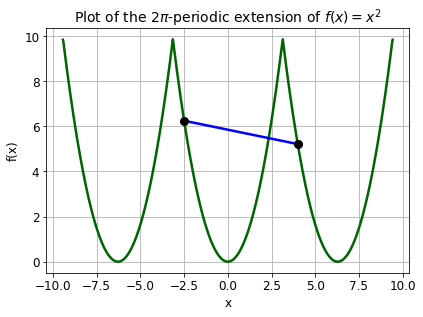
\includegraphics[width=\textwidth]{Pictures/Periodic_function_NC.png}
    \caption{2D plot of $f$}\label{fig:periodic_f}
  \end{minipage}
  \hspace{0.3cm} 
  \begin{minipage}[b]{0.37\textwidth}
    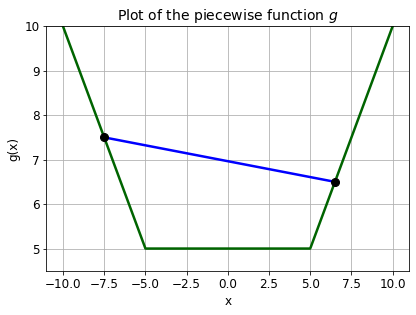
\includegraphics[width=\textwidth]{Pictures/piecewise_function_C.png}
    \caption{2D plot of $g$}\label{fig:piecewise_g}
  \end{minipage}
\end{figure}\\
The function depicted in Figure \ref{fig:periodic_f} is non-convex, because it does not satisfy the inequality given in Equation \eqref{eq:3}. This can be observed from the plot, where the line segment connecting two function values intersects the graph of the function at a point that is not one of the endpoints of the line segment. In contrast, the function shown in Figure \ref{fig:piecewise_g} is convex, because it is not possible to draw a line segment between any two function values in a way that intersects the graph of the function at a point other than the endpoints. As a result, this function satisfies Equation \eqref{eq:3}.
In the field of optimization, we frequently encounter multi-dimensional functions. These are functions with $\textbf{dom} (f)=\mathbb{R}^{n},$ where $n\in\mathbb{N}$ and $n > 1$. We consider two examples on $\mathbb{R}^2$, starting with a convex quadratic function, $f$:
\begin{equation*}\label{eq:10}\tag{2.5}
\begin{aligned}
&f(x) = \frac{1}{2}(x_{1}^{2} + 10x_{2}^{2})
\end{aligned}
\end{equation*}
Now, we compare this with a non-convex function, which we'll denote as $g$:
\begin{equation*}\label{eq:11}\tag{2.6}
\begin{aligned}
&g(x) = \frac{\sin\left(0.5x_1^2 - 0.25x_2^2 + 3\right)}{0.5 + 0.25x_1^2 + x_2^2}
\end{aligned}
\end{equation*}
Figures \ref{fig:ellipsoid_3D} and \ref{fig:Nonconvex_3D} are 3D plots of these functions.\footnote{Refer to Notebook 6, cells 4 and 5, in GitHub \cite{ThesisCode2023} for the code to create the plots.}
\begin{figure}[h]
  \centering
  \begin{minipage}[b]{0.38\textwidth}
    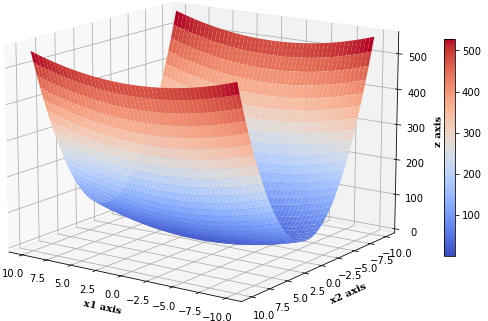
\includegraphics[width=\textwidth]{Pictures/3D plot of ellipsoid.png}
    \caption{3D plot of $f$}\label{fig:ellipsoid_3D}
  \end{minipage}
  \hspace{0.3cm} 
  \begin{minipage}[b]{0.38\textwidth}
    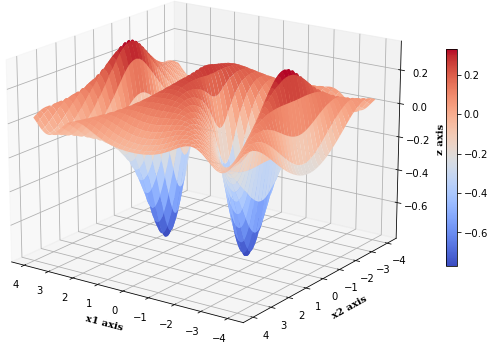
\includegraphics[width=\textwidth]{Pictures/3D plot of non convex.png}
    \caption{3D plot of $g$}\label{fig:Nonconvex_3D}
  \end{minipage}
\end{figure}\\
Visually, $f$ in Figure \ref{fig:ellipsoid_3D} represents an elliptical bowl and its graph has a parabolic shape. Clearly the optimal solution is $x^{*} = (0,0)$ with $f(x^{*}) = 0$. By visual inspection of the graph of $g$ in Figure \ref{fig:Nonconvex_3D}, one can easily verify that $g$ is non-convex, since it has many local minima and maxima. Such exploration of function properties isn't just theoretical, it has practical applications in fields like machine learning. In this domain, optimization techniques are used to train models to effectively carry out tasks. 
\newpage
In this setting, the objective function $f_0$ represents a cost function that measures the difference between the model's predictions and the true target values. The optimization problem is then to find the parameters of the model that minimize this cost function, subject to any constraints specified by the constraint functions $f_i$ and bounds $b_i$. In deep learning (a subset of machine learning), the model of choice is typically a neural network. A neural network is a computational model inspired by the human brain's own network of neurons. It consists of interconnected layers of nodes, or "neurons", and each connection has an associated weight that gets adjusted during the learning process. In the context of optimizing a cost function $f_0$, the variable $x$ represents the weights and biases of the network. The optimization problem, therefore, is to determine the values of these weights and biases that result in the best performance for a given task. This performance is evaluated using a cost function, a measure of how well the model is doing. The importance of optimization in machine learning and deep learning lies in its ability to train models that can generalize well to new data and perform well on the desired task. The optimization problem provides a framework for finding the best possible parameters of the model, given the cost function and any constraints, and is a crucial step in the training process for machine learning and deep learning models. Usually, the cost function is either convex or non-convex. Convex optimization problems can often be solved efficiently using well-established optimization algorithms, such as Deterministic Gradient Descent, often called Batch Gradient Descent (BGD). This algorithm can converge relatively quickly to a global minimum, but the convergence rate can depend on various factors, such as the dimensionality of the problem. Unfortunately, most cost functions encountered in machine learning are non-convex and high dimensional, making it hard to locate a global minimum. Luckily, it's not all bad news. In non-convex optimization, BGD has the capacity to locate at least a local minimum. In practice, such a solution is often considered satisfactory. A second challenge encountered in non-convex optimization is that the dimensionality of the problem is often very high. This makes BGD an unfavourable choice for solving the optimization as BGD requires the computation of the full gradient at every step of the algorithm. In this setting, a different class of algorithms, known as stochastic optimization algorithms, can be employed. One of these, is the famous Stochastic Gradient Descent (SGD). The key difference between between SGD and BGD, lies in their handling of high dimensionality. SGD manages this issue by computing stochastic estimates of the full gradient of the cost function during each step of the algorithm. A second advantage of SGD over BGD is its inherent stochasticity, which enables the algorithm to escape 'bad' local minima. This is a significant advantage over BGD, which can get trapped in a local minimum once it reaches one. One thing that SGD and BGD have in common, is that both are gradient-based optimization algorithms. In other words, they operate under the assumption that the cost function is differentiable. This may seem restrictive, as not all functions possess this property. Fortunately, there exists a class of optimization algorithms that aren't bound by this assumption: stochastic global optimization algorithms. These methods are especially valuable in tackling non-convex optimization problems. By employing various search strategies, they can explore the solution space more thoroughly, thereby increasing the odds of identifying the global minimum. Two such algorithms stand out: Simulated Annealing (SA) and Particle Swarm Optimization (PSO). SA is inspired by the process of annealing in metallurgy, where it's used to alter the physical properties of a material. The algorithm gradually cools the system over time, altering the solution space to help escape local minima and reach a global minimum. On the other hand, PSO draws inspiration from the social behavior of bird flocking or fish schooling. It involves a group of candidate solutions, called 'particles', moving through the solution space. Each particle adjusts its path based on its own experience and that of neighboring particles. This collective behavior helps explore the solution space more thoroughly, improving the chance of finding a global minimum. The topics introduced here will be discussed in greater detail and various applications of these topics will be showcased in this thesis.\footnote{Refer to Notebooks 1-7 on GitHub \cite{ThesisCode2023} for the implementation of the applications discussed in this thesis.}






















\clearpage\section{Basics of Convex Analysis}
One of the stepping stones in the path toward understanding stochastic gradient descent is to first understand the usual deterministic gradient descent. Gradient descent is an algorithm that is part of a family of algorithms called descent methods which are mostly applicable to unconstrained minimization problems. The simplicity of unconstrained problems allows descent methods to be fast and easy to implement. When dealing with unconstrained problems, an important assumption is the convexity of the objective function. In \ref{eq:3} a definition is given. To understand convexity in general we need to understand the notions of affine sets and convex sets. Additionally, further definitions and regularity conditions require examination. These concepts are important because the convexity assumption plays a crucial role in the convergence properties of gradient descent. 
\subsection{Convexity}
\begin{definition}
Suppose $x_{1},x_{2} \in \mathbf{R}^{n}$ with $x_{1} \neq x_{2}$. Points of the form $y = \theta x_{1} + (1-\theta) x_{2},$ where $\theta \in \mathbf{R}$, form the $\textit{line}$ passing through $x_{1}$ and $x_{2}$. The parameter value $\theta = 0$ corresponds to $y = x_{2}$ and the value $\theta = 1$ corresponds to $y = x_{1}$. The set $[x_{1},x_{2}] = \{\theta x_{1} + (1-\theta) x_{2}: \theta \in [0,1]\}$ is called the (closed) \textit{line segment} between $x_{1}$ and $x_{2}$.
\end{definition}

\begin{definition}
(\cite[21]{boyd2004convex})
A set $C \subseteq \mathbf{R}^{n}$ is \textit{affine} if the line through any two distinct points in \textit{C} lies in \textit{C}, in other words, if for any $x_{1}, x_{2} \in C$ and $\theta \in \mathbf{R}$, we have $\theta x_{1} + (1-\theta) x_{2} \in C$.
\end{definition}

\begin{definition}
(\cite[23]{boyd2004convex})
A set \textit{C} is \textit{convex} if the line segment between any two points in \textit{C} lies in \textit{C}, In other words, if for any $x_{1}, x_{2}$ $\in C$ and any $\theta$ with $0 \leq \theta \leq 1$, we have $\theta x_{1} + (1-\theta) x_{2} \in C.$
\end{definition}
\vspace*{0pt}
\begin{figure}[h!]
    \centering
        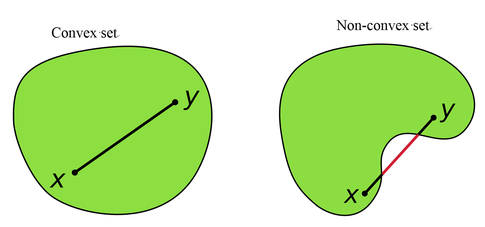
\includegraphics[width=0.45\textwidth]{Pictures/Convex ex.png}
    \caption{Example of a convex and non-convex set}
    \label{fig:conv-nonconv}
\end{figure}

\begin{definition}
(\cite[36]{boyd2004convex})
A function $f: \mathbf{R}^{n} \longrightarrow \mathbf{R}^m$ is \textit{affine} if it is a sum of a linear function and a constant, in other words, if it has a form $f(x) = Ax + b$, where $A \in \mathbf{R}^{m \times n}$ and $b \in \mathbf{R}^m$.
\end{definition}

\begin{definition}\label{definition.2.4}
(\cite[67]{boyd2004convex})
A function $f: \mathbf{R}^{n} \longrightarrow \mathbf{R}$ is convex if $\textbf{dom}(f)$ is a convex set and if for all $x,y \in \textbf{dom} \textit{f}$, and with $0 \leq \theta \leq 1$, we have 
\begin{equation*}\label{eq:4}\tag{2.1.1}
\begin{aligned}
    &f(\theta x + (1-\theta) y) \leq \theta f(x) + (1-\theta) f(y)
\end{aligned}
\end{equation*}
\end{definition}

\begin{proposition}\label{compaf}
(\cite[79]{boyd2004convex})
Suppose $f: \mathbf{R}^{n} \longrightarrow \mathbf{R}, A \in \mathbf{R}^{n\times m},$ and $b \in \mathbf{R}^{n}.$ Define $g: \mathbf{R}^{m} \longrightarrow \mathbf{R}$ by $$g(x)=f(Ax+b),$$ with $\textbf{dom} g = \{x\text{ }|\text{ }Ax+b \in \textbf{dom} (f)\}.$ Then if $f$ is convex, so is $g$.
\end{proposition}
\begin{proof}
Suppose that $f$ is convex. To show: $g$ is convex. Let $x,y \in \mathbf{R}^{n}$ and fix $\theta \in [0,1].$ Then
\begin{align*}
g(\theta x + (1-\theta)y) &= f(A(\theta x + (1-\theta)y) + b)\\
&= f(\theta(Ax - Ay) + Ay + b)\\
&= f(\theta(Ax + b) + (1 - \theta)(Ay+b))\\
&\leq \theta f(Ax + b) + (1-\theta) f(Ay + b)\\
&= \theta g(x) + (1-\theta)g(y).
\end{align*}
$x,y$ and $\theta$ are arbitrarily fixed. So the inequality holds $\forall \text{ } x,y \in \mathbf{R}^{n}$ and $\theta \in [0.1].$ Hence, $g$ is convex. 
\end{proof}
\subsection{Gradient and Optimality}
\begin{definition}[Gradient]\label{gradient}
If $f$ is differentiable along each axis, we denote 
\begin{equation*}\tag{2.2.1}
\begin{aligned}
    &\nabla f(x) \overset{def.}{=} \left(\frac{\partial f(x)}{\partial x_{1}},\ldots,\frac{\partial f(x)}{\partial x_{d}}\right)^{T} \in \mathbf{R}^{n}
\end{aligned}
\end{equation*}
the gradient vector, so that $\nabla f: \mathbf{R}^{n}\longrightarrow \mathbf{R}^{n}$ is a vector field.
\end{definition}

\begin{lemma}[First-order conditions]\label{lemma.2.1}
\textnormal{(\cite[69]{boyd2004convex})}
Suppose \textit{f} is differentiable. In other words, $\nabla f$ exists at each point in $\textbf{dom} (f)$. Then \textit{f} is convex if and only if $\textbf{dom} (f)$ is convex and
\begin{equation*}\label{eq:5}\tag{2.2.2}
\begin{aligned}
    &f(y) \geq f(x) + \nabla f(x)^{T}(y-x)
\end{aligned}
\end{equation*}
holds for all $x,y \in \textbf{dom} (f)$. This inequality is illustrated in \ref{eq:5}
\end{lemma}
The affine function $y \mapsto f(x) + \nabla f(x)^{T}(y-x)$ is, of course, the first-order Taylor approximation of $f$ near $x$. Lemma \ref{lemma.2.1} contains an if and only if statement which states that for convex functions, the first-order Taylor approximation is always a \textit{global under estimator} for the function and that the converse is also true. In the context of optimization, finding the minimum value of a function requires identifying the point at which the function attains its lowest value. Setting the gradient to zero serves as a means of locating an optimal solution, a point of inflection where the rate of change of the function is zero and the function is neither increasing nor decreasing. 
\begin{proposition}\label{eq:local_conv}
\textnormal{(\cite[7]{coursenotesML})}
If $f$ attains a local minimum at $x^{*}$ (i.e. that $f(x^{*}) \leq f(x) $ for all $x$ in some ball around $x^{*}$) then $$\nabla f(x^{*}) = 0.$$
\end{proposition}
\begin{proof}
One has for $\epsilon$ small enough and $u$ fixed
$$f(x^{*}) \leq f(x^{*} + \epsilon u) = f(x^{*}) + \epsilon \langle \nabla f(x^{*}),\text{ }u\rangle + o(\epsilon) \implies \langle \nabla f(x^{*}),\text{ }u\rangle \geq o(1) \implies \langle \nabla f(x^{*}),\text{ }u\rangle \geq 0.$$ So applying this for $u$ and $-u$ in the previous equation shows that $\langle \nabla f(x^{*}),\text{ }u\rangle = 0$ for all $u$, and hence $\nabla f(x^{*}) = 0.$
\end{proof}
\begin{proposition}\label{eq:argmin_conv}
\textnormal{(\cite[7]{coursenotesML})}
If $f$ is convex and attains a local minimum at $x^{*}$, then this local minimum is also a global minimum. If $f$ is differentiable and convex, $$x^{*} \in \underset{x}{\textnormal{argmin}}f(x) \iff \nabla f(x^{*}) = 0.$$
\end{proposition}
\begin{proof}
Let $x \in \mathbf{R}^n$ be fixed. Then there exists $0 < \theta < 1$ small enough such that $\theta x + (1-\theta)x^{*}$ is close enough to $x^{*},$ and so since it is a local minimizer $$f(x^{*}) \leq f(\theta x + (1-\theta)x^{*}) \leq \theta f(x) + (1-\theta) f(x^{*}) \implies f(x^{*}) \leq f(x).$$ Now $x \in \mathbf{R}^n$ is fixed, so this is true $\forall x \in \mathbf{R}^n$, thus $x^{*}$ is a global minimum. For the second part, the '$\Rightarrow$' implication is proven in proposition \ref{eq:local_conv}. Suppose that $\nabla f(x^{*}).$ Since the graph of $x$ is above its tangent by convexity (as stated in lemma \ref{lemma.2.1}), 
\begin{equation*}
f(x) \geq f(x^{*}) + \langle \nabla f(x^{*}),\text{ }x - x^{*}\rangle = f(x^{*})
\end{equation*}
\end{proof}
The last inequality shows that $x^{*}$ is a global minimizer of the function $f$. Hence, if \textit{f} is differentiable and convex, a necessary and sufficient condition for a point $x^{*}$ to be optimal is given by: $\nabla f(x^{*}) = 0.$ One can strengthen the convexity condition from Definition \ref{definition.2.4} and impose that the inequality is strict for $\theta \in [0,1].$ In this case $f$ is called strictly convex and $x^{*}$ is unique. Lemma \ref{lemma.2.1} will especially prove to be useful in the convergence analysis of descent methods. In many situations neither Definition \ref{definition.2.4} nor the first-order conditions are used to check the convexity of a function. For this, we need additional tools which consist of several conditions that are called second-order conditions. For this, we need the notions of the Hessian and positive semidefiniteness. 

\begin{definition}[Hessian]
(\cite[748]{adams2013calculus})
Suppose $f: \mathbf{R}^{n} \longrightarrow \mathbf{R}$ is a function such that $x\mapsto f(x)$ with the property that all second-order partial derivatives of $f$ exist, then the Hessian matrix $\mathcal{H}$ of $f$ is an $n \times n$ matrix and is given by:
\begin{equation*}
\mathcal{H}(x) = 
\begin{bmatrix}
f_{11}(x) & f_{12}(x) & \cdots & f_{1d}(x) \\
f_{21}(x) & f_{22}(x) & \cdots & f_{2d}(x) \\
\vdots             & \vdots             & \ddots & \vdots             \\
f_{d1}(x) & f_{d2}(x) & \cdots & f_{dd}(x)
\end{bmatrix}
\end{equation*}
where $f_{ij} = \frac{\partial^{2}f}{\partial x_{i}\partial x_{j}}$
\end{definition}

\begin{definition}[Positive semidefiniteness]\label{posdef}
(\cite{doi:https://doi.org/10.1002/9780470173862.app3})
Suppose that $\mathcal{V}$ is an $n \times n$ symmetric matrix, i.e., $\mathcal{V}=\mathcal{V}^{T}$, then $\mathcal{V}$ is said to be positive semidefinite if 
\begin{equation*}\label{eq:6}\tag{2.2.3}
\begin{aligned}
    &x^{T} \mathcal{V} x \geq 0 
\end{aligned}
\end{equation*}
for all $x \in \mathbf{R}^{n}$. Notation: $\mathcal{V} \succeq 0.$
\end{definition}
\begin{lemma}[Second-order conditions]\label{second-ord-cond}
(\cite[71]{boyd2004convex})
We now assume that f is twice differentiable, that is, its Hessian or second derivative $\nabla^{2}f$ exists at each point in $\textbf{dom} (f)$. Then f is convex if and only if $\textbf{dom} (f)$ is convex and its Hessian is positive semidefinite: for all $x \in \textbf{dom} (f),$ 
\begin{equation*}\label{eq:9}\tag{2.2.4}
\begin{aligned}
    &\nabla^{2}f(x) \succeq 0.
\end{aligned}
\end{equation*}
\end{lemma}
\begin{proof}
    
\end{proof}

\newpage
\subsection{Unconstrained Minimization Problems}
In this section unconstrained minimization problems will be discussed in more detail. Descent methods play a big role in solving these problems. Descent methods are optimization algorithms for solving the unconstrained minimization problem 
\begin{equation*}\label{eq:8}\tag{2.3.1}
\begin{aligned}
    &\text{minimize} \text{ } f(x)\\ 
    &\textbf{dom} (f) = \mathbf{R}^n
\end{aligned}
\end{equation*}
where $f: \mathbf{R}^{n} \longrightarrow \mathbf{R}$ is the objective function. The true optimal solution to this problem may be a set of $x^{*} \in D$ of all optimal points in $D$, rather than a single minimum. In general, there might be no solution to the optimization \eqref{eq:8}. This is the case if $f$ is unbounded below, for example, if $f(x) = -x^{2}$ in which case the minimum value is $-\infty.$ It can also be the case that $f$ does not grow at infinity, for example if $f(x) = e^{-x}$, for which min$f$ = 0, but there is no minimizer. The task of any good optimization problem is to find globally optimal solutions if they exist. The objective function could be continuous, discontinuous, linear, non-linear, and convex. Problems with convex objectives are easiest to work with, since in that case, the problem is solvable and optimal solutions in which the function attains the global minimum can be found. The best case scenario is when there is one unique optimal solution $x^{*}$. For convex functions, solving the unconstrained minimization problem is the same as finding a solution to \eqref{eq:argmin_conv}. Since there are $d$ variables $(x_{1},\ldots,x_{d}),$ a system of $d$ equations needs to be solved. This can be a difficult process to solve analytically, especially in the case of non-linear functions and when $d$ is large. Therefore, usually, iterative algorithms are consulted. Such an algorithm computes a sequence of points called a minimizing sequence for \ref{eq:8}. First a starting point $x^{(0)}$ is chosen and in the following iterations the algorithm computes $x^{(1)}, x^{(2)},\ldots$ such that $f(x^{(k)}) \longrightarrow p^{*}=f(x^{*})$ as $k \longrightarrow \infty$. The key consideration when selecting $x^{(0)}$ is addressed by the following definition:
\begin{definition}[Sublevel sets]
\cite[75]{boyd2004convex}  
The $\alpha-\textit{sublevel set}$ of a function $f: \mathbf{R}^{n} \longrightarrow \mathbf{R}$ is defined as $$C_{\alpha} = \{x \in \textbf{dom} (f) \text{ }|\text{ } f(x) \leq \alpha\}.$$
\end{definition}
\begin{remark}
\cite[75]{boyd2004convex}  
Sublevel sets of a convex function are convex, for any value of $\alpha$.
\end{remark}
\begin{proof}
Suppose that the function $f$ is convex. Let $x,y \in C_{\alpha}$ and fix $\theta \in [0,1]$. Then $$f(\theta x + (1-\theta)y) \leq \theta f(x) + (1-\theta)f(y) \leq \theta \alpha + (1-\theta)\alpha = \alpha$$
Since $x,y$ and $\theta$ are arbitrarily chosen, the statement holds for all $x,y \in C_{\alpha}$ and $\theta \in [0,1]$.
\end{proof} 
Now trivially it is required that $x^{(0)} \in \textbf{dom} (f)$, and as discussed in \cite[457]{boyd2004convex} the sublevel set 
\begin{equation*}\label{eq:13}\tag{2.3.2}
\begin{aligned}
    &S = \{x \in \textbf{dom} (f) \text{ }|\text{ } f(x) \leq f(x^{0})\}
\end{aligned}
\end{equation*}
must be closed. This condition is satisfied for all $x^{(0)} \in \textbf{dom} (f)$ if the function $f$ is closed. We call $f$ closed if all its sublevel sets are closed. Continuous functions with $\textbf{dom} (f) = \mathbf{R}^{n}$ are closed, so if $\textbf{dom} (f) = \mathbf{R}^{n}$, the initial sublevel set condition \ref{eq:13} is satisfied by any $x^{(0)}$. In this thesis, most of the functions that are examined are continuous functions on $\mathbf{R}^{n}.$ Hence, we have the freedom to choose any particular $x^{(0)}$ as a starting point. Iterative algorithms that solve problem \eqref{eq:8} terminate whenever $f(x^{(k)}) - p^{*} \leq \epsilon$ for some tolerance $\epsilon$ small and $k \in \mathbb{N}$.









\clearpage\section{Gradient Descent Algorithm}\label{sec: GD}
\subsection{Gradient Descent}
Gradient descent is part of a family of algorithms called descent methods. With descent methods a minimizing sequence $(x^{(k)})$ with $k = 1,\ldots$ can be generated where $$x^{(k+1)} = x^{(k)} + \tau^{(k)} \Delta x^{(k)}$$ Here $\tau^{(k)} > 0$ is called the step size and $\Delta x^{(k)}$ is called the search direction. The superscripts $k=0,1\ldots$ denote the iteration numbers. Since the goal is to eventually minimize the function $f$ in \eqref{eq:8}, it should hold that $f(x^{(k+1)}) < f(x^{(k)})$ for every $k \in \mathbb{N}$ considered, until an optimal solution is reached. To achieve a decrease in the function value in every iteration, the search direction needs to satisfy the following strict inequality: $$\nabla f(x^{(k)})^{T} \Delta x^{(k)} < 0.$$ By definition, the gradient of the function at the current iteration, say $\nabla f(x^{(k)})$, points in the direction of the steepest increase of the function. To minimize $f$, the search direction $\Delta x^{(k)}$ should be chosen to point in the opposite direction. This means that the angle between the gradient and the search direction should be acute, and as a result, the inner product between $\nabla f(x^{(k)})$ and $\Delta x^{(k)}$ should be less than 0. As stated in \cite[464]{boyd2004convex}, a general descent method consists of the following stages: 
\begin{algorithm}
\caption{\textit{General descent method}}
\begin{algorithmic}
\State \textbf{Given} a starting point $x \in \textbf{dom} (f)$.
\vspace{0.03cm}
\State \textbf{repeat}\\
\begin{enumerate}
    \item Determine a descent direction $\Delta x.$
    \item \textit{Line search.} Choose a step size $\tau > 0$.
    \item \textit{Update.} $x := x + \tau \Delta x.$
\end{enumerate}
\State \textbf{until} stopping criterion is satisfied.
\end{algorithmic}
\end{algorithm}\\
The negative gradient $\Delta x = -\nabla f(x)$ is a natural choice for the search direction. The resulting algorithm is called the \textit{gradient descent method.} As stated in \cite[466]{boyd2004convex}, the gradient descent method consists of the following stages:
\begin{algorithm}
\caption{\textit{Gradient descent method}}\label{Pseudocode_GD}
\begin{algorithmic}
\State \textbf{Given} a starting point $x \in \textbf{dom} (f)$.
\vspace{0.03cm}
\State \textbf{repeat}\\
\begin{enumerate}
    \item $\Delta x := -\nabla f(x).$
    \item \textit{Line search.} Choose a step size $\tau > 0.$
    \item \textit{Update.} $x := x + \tau \Delta x.$
\end{enumerate}
\State \textbf{until} stopping criterion is satisfied.
\end{algorithmic}
\end{algorithm}\\
The second step in the repeat block is known as the \textit{line search}. The step size $\tau$ determines the next vector $x$. We consider two approaches for determining the step size, namely fixed step size and line search. In the fixed step size method, the same step size $\tau$ is used for every iteration until the stopping criterion is met. On the other hand, the line search method adjusts the step size at each iteration to ensure that the algorithm progresses toward the minimum without overshooting it. Specifically, the line search method searches for the optimal step size that minimizes the cost function along the descent direction. This allows the algorithm to take larger steps when the slope is steep and smaller steps when the slope is flat. The stopping criterion is often checked immediately after the descent direction $\Delta x$ is computed. The stopping criterion is of the form $||\nabla f(x)||_{2} \leq \eta,$ where $\eta$ is small and positive. 

\subsection{Convergence Analysis of Gradient Descent}
Two different methods for choosing the step size have been briefly discussed. It is important to prove that the gradient descent method converges for both. To solve the problem $\nabla f(x^{*}) = 0$ via gradient descent, we start with some initial guess $x^{(0)},$ and then the algorithm produces a sequence $\{x^{(k)}\}$ where hopefully the sequence converges to $x^{*}$, meaning $||x^{(k)}-x^{*}||_{2} \rightarrow 0$ as $k \rightarrow \infty$ where $||\cdot||_{2}$ is the Euclidean norm.
\subsubsection{Convergence analysis of gradient descent with fixed step size}
For gradient-based optimization methods like gradient descent, a key issue is choosing an appropriate step size. In a fixed step size method, the step size is chosen in advance and remains constant throughout the optimization process. This can lead to two problems: if the step size is too small, the algorithm may take too many iterations to converge to the minimum, while if the step size is too large, the algorithm may overshoot the minimum and diverge. The question of whether or not gradient descent converges in the case of a fixed step size $\tau$, boils down to finding an appropriate interval from which $\tau$ can be chosen. Usually, the correct range of step sizes is determined by the Lipschitz constant of $\nabla f(x)$ and the strong convexity constant $\alpha.$ In the convergence proof of gradient descent, an important assumption is that the objective function has Lipschitz continuous gradients. These functions are called smooth functions.
\begin{definition}
\cite[8]{GDlips}
A differentiable function $f:\mathbb{R}^{n}\longrightarrow\mathbb{R}$ is called smooth $\iff$ it has a Lipschitz continuous gradient, i.e., $\iff$ $\exists L < \infty$ such that
\begin{equation*}\label{eq:14}\tag{4.2.1.1}
\begin{aligned}
    &||\nabla f(x) - \nabla f(z)||_{2} \leq L||x-z||_{2},\text{ } \forall x, z \in \mathbb{R}^{n}.
\end{aligned}
\end{equation*}
\end{definition}
Later on, it will become clear why $L$ plays a crucial role in determining the step size $\tau.$ One may naturally wonder  how to determine $L.$ While it is not always possible to determine the Lipschitz constant of the gradient for every smooth function, the following remark provides a method to find $L.$
\begin{remark}\label{findL}
\cite[10]{GDlips}
If $f:\mathbb{R}^{n}\longrightarrow\mathbb{R}$ is twice differentiable and if there exists $L < \infty$ such that its Hessian matrix has a bounded spectral norm\footnote{See \ref{spectral norm} for theorem about the spectral norm.}:
\begin{equation*}\label{eq:15}\tag{4.2.1.2}
\begin{aligned}
    &\vertiii{\nabla^{2} f(x)}_{2} \leq L,\text{ } \forall x \in \mathbb{R}^{n}
\end{aligned}
\end{equation*}
then $f$ has a Lipschitz continuous gradient with Lipschitz constant L. 
\end{remark}
\begin{proof}
Using the fundamental theorem of calculus and the triangle inequality:
\begin{align*}
&\left\Vert\nabla f(x) - \nabla f(z)\right\Vert_{2}
=\left\Vert\int_{0}^{1} \nabla^{2} f(x + t(z-x))\,dt(z-x)\right\Vert_{2}\\
&\leq \left(\int_{0}^{1} \vertiii{\nabla^{2} f(x + t(z-x))}_{2} \,dt\right) ||x-z||_{2} \leq \left(\int_{0}^{1} L \,dt\right) ||x-z||_{2} = L\text{ }||x-z||_{2}\qedhere
\end{align*}
\end{proof}
Another assumption for the convergence proof is that the objective function $f$ is strongly convex. As the name suggest this assumption is "stronger" than mere convexity. In fact strong convexity implies strict convexity which implies convexity. 
\begin{definition}
\cite[459]{boyd2004convex}
If $f:\mathbb{R}^{n}\longrightarrow\mathbb{R}$ is twice differentiable. Then $f$ is called strongly convex on $\textbf{dom}(f)=\mathbb{R}^{n},$ if there exists an $\alpha > 0$ such that
\begin{equation*}\label{eq:16}\tag{4.2.1.3}
\begin{aligned}
    &\nabla^{2} f(x) \succcurlyeq \alpha I \text{ } \text{ }\forall x \in \textbf{dom}(f)
\end{aligned}
\end{equation*}
\end{definition}
Strong convexity has several interesting consequences. For $x,y \in \textbf{dom}(f)$ we have
$$f(y) = f(x) + \nabla f(x)^{T}(y-x) + \frac{1}{2} (y-x)^{T}\nabla^{2} f(z) (y-x)$$
for some $z$ on the line segment $[x, y].$ By strong convexity assumption \eqref{eq:16} we get that the last term on the right hand side is at least $(\alpha/2)||y-x||^{2}_{2}.$ We obtain first-order characterization \eqref{eq:17}:
\begin{equation*}\label{eq:17}\tag{4.2.1.4}
\begin{aligned}
    &f(y) \geq f(x) + \nabla f(x)^{T}(y-x) + \frac{\alpha}{2}||y-x||^{2}_{2}
\end{aligned}
\end{equation*}
for all $x,y \in \textbf{dom}(f)$. For $\alpha=0$, the lower bound for convexity is recovered. Proposition \ref{pf_gd_sc_L} below gives an upper bound for the step size $\tau$ for which convergence is ensured.
\begin{proposition}\label{pf_gd_sc_L}
Let $f: \mathbb{R}^{n}\longrightarrow \mathbb{R}$ be $\alpha$-strongly convex and differentiable on $\textbf{dom}(f) = \mathbb{R}^{n}.$ Furthermore, suppose that $f$ is smooth on $\textbf{dom}(f)= \mathbb{R}^{n}$, i.e., $\nabla f$ is Lipschitz with Lipschitz constant $L$ and that the optimum value $f^{*} = \textnormal{min}_{x}(f(x))$ is finite and attained at $x^{*}$ such that $\nabla f(x^{*})=0.$ Then $||x^{(k+1)}-x^{*}|| \rightarrow 0$ as $k \rightarrow \infty$ if $\tau < 2\alpha/L^{2}$ where $\tau$ is the step size. $||\cdot||$ is the Euclidean norm. 
\end{proposition}
\begin{proof}
Goal: Find $0\leq C < 1$ such that $||x^{(k+1)} - x^{*}|| \leq C||x^{(k)} - x^{*}||.$ If such a $C$ exists then inductively $||x^{(k+1)} - x^{*}|| \leq C||x^{(k)} - x^{*}|| \leq C^{2}||x^{(k-1)} - x^{*}|| \leq \ldots \leq C^{k+1}||x^{(0)} - x^{*}||$, which means that as $k\rightarrow \infty$ $||x^{(k+1)} - x^{*}|| \rightarrow 0.$ Now since $f$ is $\alpha$-strongly convex:
\begin{align}
    &f(y) - f(x) \geq \langle \nabla f(x),\text{ } y-x\rangle + \frac{\alpha}{2}||y-x||^{2} \text{ }\text{ } \forall x,y \in \mathbb{R}^{n}\text{,} \text{ } \text{hence} \nonumber\\
    &f(x^{(k)}) - f(x^{*}) \geq \langle \nabla f(x^{*}),\text{ } x^{(k)}-x^{*}\rangle + \frac{\alpha}{2}||x^{(k)}-x^{*}||^{2}\nonumber\\
    &f(x^{*}) - f(x^{(k)}) \geq \langle \nabla f(x^{(k)}),\text{ } x^{*}-x^{(k)}\rangle + \frac{\alpha}{2}||x^{*}-x^{(k)}||^{2}\nonumber
\end{align}
Summing these inequalities and using $\nabla f(x^{*}) = 0$ yields:
\begin{align}
    &\langle \nabla f(x^{(k)}) - \nabla f(x^{*}),\text{ } x^{(k)} - x^{*}\rangle = \langle \nabla f(x^{(k)}),\text{ } x^{(k)} - x^{*}\rangle \geq \alpha ||x^{(k)} - x^{*}||^{2}.
\end{align}
$\nabla f$ is Lipschitz with Lipschitz constant $L$, so we get:
\begin{align}
    &||\nabla f(x) - \nabla f(y)|| \leq L||x-y||,\text{ } \forall x, y \in \mathbb{R}^{n} \implies ||\nabla f(x^{(k)}) - \nabla f(x^{*})|| \leq L||x^{(k)}-x^{*}||
\end{align}
Now choose $\tau > 0,$ then:
\begin{align}
||x^{(k+1)}-x^{*}||^{2}
    &= ||x^{(k)}-x^{*}-\tau \nabla f(x^{(k)})||^{2} = ||x^{(k)}-x^{*}-\tau (\nabla f(x^{(k)})-\nabla f(x^{*}))||^{2}\nonumber\\
    &= ||x^{(k)}-x^{*}||^{2} + \tau^{2}||\nabla f(x^{(k)})-\nabla f(x^{*})||^{2} - 2\tau \langle x^{(k)}-x^{*},\text{ } \nabla f(x^{(k)})-\nabla f(x^{*})\rangle\\
    &\leq ||x^{(k)}-x^{*}||^{2} + \tau^{2}L^{2}||x^{(k)}-x^{*}||^{2} - 2\alpha \tau||x^{(k)}-x^{*}||^{2}\nonumber\\
    &= \left(1+\tau^{2}L^{2}-2\alpha \tau \right)||x^{(k)}-x^{*}||^{2} = C||x^{(k)}-x^{*}||^{2}
\end{align}
where we used inequalities (1) and (2) to bound (3) by (4) and have set $C = 1+\tau^{2}L^{2}-2\alpha \tau.$\\ Now $0\leq C<1 \iff$ 0 $\leq 1+\tau^{2}L^{2}-2\alpha \tau < 1 \implies -1 \leq \tau\left(\tau L^{2}-2\alpha \right) < 0 \implies \tau L^{2}-2\alpha < 0 \implies \tau < 2\alpha/L^{2}.$ 
\end{proof}
We observe that $\tau < 2\alpha / L^{2}$ is a sufficient condition for convergence of gradient descent, however, it is not a necessary condition. There are many cases where gradient descent converges even when $\tau \geq 2\alpha / L^{2}$. Other researchers have found a different bound for the step size. For example in \cite[10]{GDandLS}, the bound $\tau \leq 2/(\alpha+L)$ is given, where the assumptions for $f$ are the same as for Proposition \ref{pf_gd_sc_L}. It will depend on the problem at hand which of the bounds is less tight. Both bounds ensure convergence, so choosing the sharper bound secures faster convergence. Generally, $\tau$ can be chosen such that $\tau < \max\{2\alpha / L^{2},\text{ } 2/(\alpha+L)\}$ is satisfied. In both cases, the algorithm's running time is represented by $O(C^{k})$, which is known for its exponential speed. This phenomenon is known as \textit{linear convergence}, which can be observed as a straight line when plotted on a logarithmic scale. Specifically, plotting the iterations on the x-axis and the difference in function values on the y-axis with respect to the final iterate results in a straight line. Another known bound for the step size is the bound $\tau \leq 1/L.$ The difference between this bound and the prior bounds is that in this case, the assumption of strong convexity is relaxed, and only convexity is needed. See Proposition \ref{pf_gd_c_L} below, and its proof in \cite[9]{GDandLS}.
\begin{proposition}\label{pf_gd_c_L}
\textnormal{\cite[9]{GDandLS}}
Let $f: \mathbb{R}^{n}\longrightarrow \mathbb{R}$ be convex and differentiable on $\textbf{dom}(f)= \mathbb{R}^{n}.$ Furthermore, suppose that $f$ is smooth on $\textbf{dom}(f) = \mathbb{R}^{n}$, i.e., $\nabla f$ is Lipschitz with Lipschitz constant $L$ and that the optimum value $f^{*} = \textnormal{min}_{x}(f(x))$ is finite and attained at $x^{*}$ such that $\nabla f(x^{*})=0.$ Then gradient descent with fixed step size $\tau \leq 1/L$ satisfies $f(x^{(k)})-f(x^{*}) \leq \frac{||x^{(0)}-x^{*}||^{2}}{2\tau k}.$ 
\end{proposition}
When dealing with this particular case, the running time of the algorithm is represented by $O(1/k)$, which is comparatively slower than $O(C^{k})$. Additionally, it is observed that $\max\{2\alpha / L^{2},\text{ } 2/(\alpha+L)\} > 1/L.$ Therefore, if the objective function is strongly convex, utilizing $\max\{2\alpha / L^{2},\text{ } 2/(\alpha+L)\}$ as the bound for $\tau$ ensures faster convergence. However, it is worth noting that in cases where determining strong convexity is difficult, one can always choose $1/L$. Moreover, most convex functions are not strongly convex. Only a small subset of convex functions are strongly convex.
\subsubsection{Convergence analysis of gradient descent with backtracking line search}
Backtracking line search is an adaptive step size method that computes a different step size for each descent iteration. For a general descent method, we are given a starting vector $x$ and a search direction $\Delta x.$ The task of the line search is to determine a step size $\tau>0,$ that adequately reduces the objective function $f:\mathbb{R}^{n}\longrightarrow\mathbb{R}$ (assumed to have Lipschitz continious gradient). In other words, to find a value of $\tau$ that reduces $f(x+\tau\Delta x)$ relative to $f(x).$ The algorithm depends on two constants, $\alpha,\beta$ with $\alpha\in(0,0.5)$ and $\beta\in(0,1).$ The line search starts with a unit step size $\tau=1$ and iteratively shrinks it with a factor $\beta$, until the stopping condition  
\begin{equation*}\tag{4.2.2.1}\label{line_stopping_condition}
f(x+\tau\Delta x)\leq f(x) + \alpha\tau\nabla f(x)^{T}\Delta x
\end{equation*}
is met.
Figure \ref{fig:line_search} illustrates the main idea of the backtracking algorithm. The inequality given in \eqref{line_stopping_condition} ensures that the backtracking algorithm results in an improvement in the objective function value at the next step \cite{boyd2004convex}. The pseudo-code for gradient descent using backtracking line search, where $\Delta x = -\nabla f(x),$ is given in Algorithm \ref{Pseudo_backtrack}. The stopping condition of the outer loop allows us to approach a local or global minimum, while the stopping condition of the inner loop checks if inequality \eqref{line_stopping_condition} holds.
\begin{algorithm}
\caption{\textit{Gradient descent with backtracking line search}}\label{Pseudo_backtrack}
\begin{algorithmic}
\vspace{0.05cm}
\State \textbf{given} a starting point $x\in\textbf{dom} (f),\text{ } \alpha\in(0,0.5),\text{ }\beta\in(0,1).$\\
\textbf{while} stopping criterion $\left\Vert\nabla f(x)\right\Vert_{2}\leq \eta$ is not satisfied \textbf{do}\\
\hspace{0.3cm} \textit{Line search,} set $\tau:=1$\\
\hspace{1.1cm} \textbf{while} $f(x-\tau\nabla f(x))> f(x) - \alpha\tau\left\Vert\nabla f(x)\right\Vert_{2}$ \textbf{do}\\
\quad \hspace{1.2cm} $\tau:=\beta\tau$\\
\hspace{1.1cm} \textbf{end while}\\
\hspace{0.3cm} \textit{Update} $x:=x-\tau\nabla f(x).$\\
\textbf{end while}
\vspace{0.05cm}
\end{algorithmic}
\end{algorithm}\\
Now if inequality \eqref{line_stopping_condition} holds for $\Delta x = -\nabla f(x),$ then 
\begin{equation*}\tag{4.2.2.2}\label{objective_imp}
f(x-\tau\nabla f(x))\leq f(x) - \alpha\tau\left\Vert\nabla f(x)\right\Vert_{2} \leq f(x)
\end{equation*}
holds, which shows that the algorithm indeed results in an improvement in the objective function.
\begin{figure}[h!]
    \centering
        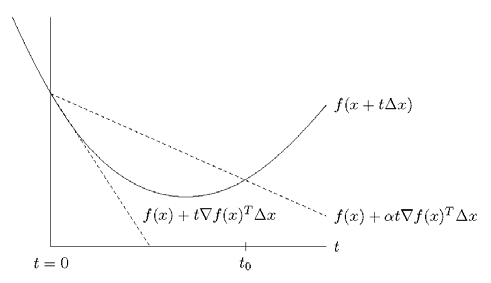
\includegraphics[width=0.5\textwidth]{Pictures/line_search.png}
    \caption{\textit{Backtracking line search.} 
 The lower dashed line shows the linear extrapolation of $f,$ and the upper dashed line has a slope a factor of $\alpha$ smaller. The stopping condition is that $f$ lies below the upper dashed line.}\label{fig:line_search}
\end{figure}
\begin{proposition}\textnormal{\cite[10]{GDandLS}}\label{pf_gd_bt}
Let $f:\mathbb{R}^{n}\longrightarrow\mathbb{R}$ be convex and differentiable. Suppose that $f$ is smooth with Lipschitz constant $L > 0.$ Then gradient descent with backtracking line search satisfies $f(x^{(k)})-f(x^{*}) \leq \frac{||x^{(0)}-x^{*}||^{2}}{2\tau_{min} k},$ where $\tau_{min} = \min\{1,\frac{\beta}{L}\}.$ If $f$ is also strongly convex, then the algorithm satisfies $f(x^{(k)})-f(x^{*}) \leq C^{k}\frac{L}{2}||x^{(0)}-x^{*}||^{2},$ where $C\in(0,1).$
\end{proposition}
For the proof of Proposition \ref{pf_gd_bt}, please refer to the notes by Geoff Gordon and Ryan Tibshirani \cite[10]{GDandLS}. Proposition \ref{pf_gd_bt} allows us to conclude that Algorithm \ref{Pseudo_backtrack} exhibits a running time of $O(1/k)$ for convex objectives and of $O(C^{k})$ for strongly convex objectives. This means that $f(x^{(k)}) \xrightarrow{k\rightarrow\infty} f(x^{*})$ is achieved faster, at exponential rate, for strongly convex objective functions. 
\clearpage\section{Stochastic optimization}
\subsection{Machine learning}
\subsubsection{Motivation}
Stochastic optimization is routinely used in machine learning. Machine learning is a field that enables computers to learn from data and improve their performance. Learning methodologies in machine learning generally fall under one of three primary paradigms: supervised learning, unsupervised learning, and reinforcement learning \cite[101-105]{Goodfellow-et-al-2016}. This thesis will focus on the approach of supervised learning. As suggested by the name, this method involves training a machine learning model using labeled data. The model is exposed to training examples composed of inputs and their corresponding desired outputs, which are provided by a human supervisor. The objective is to formulate a general rule that can effectively map these inputs to the correct outputs. In this context, the model is equipped with a set of parameters, commonly referred to as weights and biases, and denoted as $\theta \in \mathbb{R}^{p}$, which are randomly initialized before the training process begins. The key to achieving the goal of accurately mapping inputs to their intended outputs lies in identifying an optimal set of these parameters. Once the parameters are initialized, inputs are fed into the model, which in turn generates corresponding outputs. These outputs represent the model's predictions of the true values. Performance is measured using a loss function, which quantifies the difference between the predicted outputs and the true values. When dealing with an entire dataset, we calculate a cost or objective function, which is typically the average of all individual losses across the dataset. The aim of supervised learning is to adjust the parameters $\theta$ to minimize this cost function, thereby improving overall model performance. To achieve this, Stochastic Gradient Descent (SGD) methods are commonly employed, especially when dealing with large datasets. The details of these concepts and their implementation in the optimization of neural networks will be discussed in the subsequent sections.
\subsubsection{Basics of Supervised Learning and Neural Networks}\label{Basic_of_SL_FFNN}
\paragraph{Supervised Learning}
Supervised learning uses labeled data, consisting of input-output pairs $(x, y)$. The underlying relationship between the inputs and outputs is often represented by a 'true function' $f: \mathbb{R}^{d_{1}}\rightarrow \mathbb{R}^{d_{2}}$, where $d_{1}, d_{2} \in \mathbb{Z}_{+},$ such that $f(x)=y$ \cite{bishop2006}. However, in practice, this function is unknown, and our goal is to approximate it as closely as possible using a model. In the context of supervised learning, a model is represented by a function $f_{m}$ which takes an input $x$ and parameters $\theta$ to produce a predicted output $\hat{y}=f_{m}(x, \theta)$ \cite{Goodfellow-et-al-2016}. To approximate $f,$ the model $f_{m},$ is trained on a subset of the data that is available, $\{(x^{(1)},y^{(1)}),\ldots,(x^{(n)},y^{(n)})\}$, where $x^{(i)}$ is an input and $y^{(i)}$ is the corresponding label we wish to get from $f(x^{(i)}) \text{ } \text{ }\forall i\in\{1,\ldots n\}$. The parameters $\theta$ are adjusted such that the model's outputs $\hat{y}$ closely align with the true outputs $y$ from the training data. This alignment is quantified by a cost function, which measures the average discrepancy between the model's predictions and the actual outputs over the entire dataset. The goal of the training process is not only to minimize this cost on the training data, but, more importantly, to modify the model such that it generalizes well to unseen data. This is known as the model's capacity for generalization. The better a model can generalize, the more accurate its predictions will be when presented with new data outside of the training set \cite{james2013}.

\paragraph{Feed-forward Neural Networks}\label{Basic_of_FFNN}
Feed-forward neural networks are a common type of model used in supervised learning. They attempt to approximate the unknown function $f: x \mapsto y$ by defining a function $f_{m}: (x,\theta) \mapsto \hat{y}$, where $\hat{y}$ is the predicted output, $x$ is the input, and $\theta$ represents the model's parameters (the weights and biases of the neurons in the network). The network consists of multiple layers, including input, hidden, and output layers. Each layer contains a number of neurons that receive inputs from the previous layer, apply a weighted sum with a bias term, and then apply an activation function. This activation function introduces non-linearity into the model, enabling it to learn and represent complex patterns in the data. The training process involves adjusting the parameters $\theta$ to minimize the cost function. This is done using an optimization algorithm, such as stochastic gradient descent, which iteratively updates the weights and biases based on the gradients of the loss function with respect to these parameters. A detailed mathematical exploration of stochastic gradient descent will be provided later in the document. Afterwards, the function of each layer in a feed-forward neural network will be discussed, particularly within the context of a specific application of these networks.
\newpage
\subsection{Minimizing Sums and Expectation}
In the context of supervised learning, we aim to approximate the unknown function $f: \mathbb{R}^{d_{1}}\rightarrow \mathbb{R}^{d_{2}}$. This function maps each input $x$ to an output $y$. We approximate $f$ using a model function, denoted $f_{m}: \mathbb{R}^{d_{1}}\times \mathbb{R}^{p}\rightarrow \mathbb{R}^{d_{2}}$. The model function $f_{m}$ takes an input $x$ and a set of parameters $\theta$ and produces an output $\hat{y}$, which is our prediction of the true output $y$. We have at our disposal an initialized set of parameters $\theta$ and a training set of $n$ examples $T=\{(x^{(1)},y^{(1)}),\ldots,(x^{(n)},y^{(n)})\},$ where $x^{(i)} \in \mathbb{R}^{d_{1}}$ and $y^{(i)} \in \mathbb{R}^{d_{2}} \text{ } \text{ } \forall i\in\{1,\ldots,n\}.$ We assume that there is an unknown joint probability distribution $P_{XY}:\Omega\rightarrow [0,1],$ where $\Omega = \mathbb{R}^{d_{1}} \times \mathbb{R}^{d_{2}}$ is the sample space. Furthermore, we assume that the training examples $(x^{(1)},y^{(1)}),\ldots,(x^{(n)},y^{(n)})$ are drawn i.i.d. from $P_{XY}.$ We also assume that we are given a non-negative real-valued loss function $L(\hat{y},y),$ which measures the difference between the prediction $\hat{y}$ and the true outcome $y.$ As discussed in \cite[20]{coursenotesML}, the cost $F$ associated with the function $f_{m}$ is then defined as an expectation of the loss function $L$. To approximate $f$ by $f_{m},$ we need to minimize the cost function. The optimization problem can then be expressed as:  
\begin{equation*}\label{min_expectations}\tag{5.2.1}
\underset{\theta \in \mathbb{R}^{p}}{\text{min}} F(\theta) \overset{\text{def.}}{=} \mathbb{E}_{(x,y)\sim P_{XY}}[L(f_{m}(x, \theta), y)] = \int_{\Omega} L(f_{m}(x, \theta), y) dP_{XY}(x,y).
\end{equation*}
While minimizing expectations is a general framework that allows us to account for uncertainty in the data, the cost function $F$ cannot be computed, because the joint distribution $P_{XY}$ is unknown to the learning algorithm. However, we can calculate an approximation to the cost function, known as the empirical cost and denote it by $F_{m}$. This is achieved by averaging the values of the loss function across the entire training set. The optimization problem can then be expressed as:
\begin{equation*}\label{largesums}\tag{5.2.2}
\underset{\theta \in \mathbb{R}^{p}}{\text{min}} F_{m}(\theta) \overset{\text{def.}}{=} \frac{1}{n} \sum_{i=1}^{n}L(f_{m}(x^{(i)}, \theta), y^{(i)}).
\end{equation*}
Problem \eqref{largesums} is a special case of \eqref{min_expectations} when replacing the true distribution $P_{XY}:\Omega\rightarrow[0,1]$ with the joint Empirical Cumulative Distribution (ECDF) $\hat{P}_{XY_{n}}:T\rightarrow[0,1],$ defined by the training set $T.$
\begin{definition}(\cite[1]{CastroNotes})\label{ECDF}
Let $(X^{(1)},Y^{(1)}),\ldots,(X^{(n)},Y^{(n)})$ be a sample of $n$ data points, where each $X^{(i)} = (X^{(i)}_{1},\ldots,X^{(i)}_{d_{1}})$ and $Y^{(i)} = (Y^{(i)}_{1},\ldots,Y^{(i)}_{d_{2}})$ are vector-valued random variables. The sequence $\left\{(X^{(i)},Y^{(i)})\right\}_{i=1}^{n}$ is assumed to be independent and identically distributed (i.i.d.) according to the joint distribution $P_{XY}.$ We denote, $P_{XY}(x,y)=\mathbb{P}\left(X_{1}\leq x_{1},\ldots,X_{d_{1}}\leq x_{d_{1}},Y_{1}\leq y_{1},\ldots,Y_{d_{2}}\leq y_{d_{2}}\right).$ 
The joint ECDF for $P_{XY}$ is defined as
\begin{equation*}\tag{5.2.3}
\hat{P}_{XY_{n}}(x,y) = \frac{1}{n} \sum_{i=1}^{n} \mathbbm{1}\left\{X_{1}^{(i)}\leq x_{1},\ldots,X_{d_{1}}^{(i)}\leq x_{d_{1}},Y_{1}^{(i)}\leq y_{1},\ldots,Y_{d_{2}}^{(i)}\leq y_{d_{2}}\right\}.
\end{equation*}
\footnote{Here, $\mathbbm{1}$ is the indicator function, which is one if the condition inside the brackets is true and zero otherwise.}
\end{definition}
The joint ECDF takes the form of a step function, which by jumps by $1/n$ at each of the observed data points $(X^{(i)}, Y^{(i)})$ Rui Castro states in his notes about the univariate ECDF, "Clearly the ECDF seems to be a sensible estimator for the underlying distribution."\cite{CastroNotes} The following theorem provides a justification to use $\hat{P}_{n}$ as an estimator for $P$ in the univariate case:
\begin{theorem}[Glivenko-Cantelli Lemma]\textnormal{(\cite[2]{CastroNotes})}\label{Glivenko}
For a sequence of univariate random variables, the empirical distribution converges uniformly to $P(x),$ namely
\begin{equation*}\tag{5.2.4}
\left\Vert \hat{P}_{n} - P\right\Vert_{\infty} = \underset{x\in \mathbb{R}}{\sup}\left|\hat{P}_{n}(x) - P(x)\right|\xrightarrow{a.s.} 0,
\end{equation*}
as $n\rightarrow\infty,$ where the superscript a.s. denotes convergence almost surely.
\end{theorem}
For a comprehensive proof of this theorem, please refer to Castro's work \cite[8]{CastroNotes}. Our data involves multivariate ECDFs, therefore we have to seek for a multidimensional extension of the Glivenko-Cantelli theorem. Specifically, the Vapnik-Chervonenkis inequality serves as a suitable generalization. The theorem and its proof is presented in an abstract form in \cite[4-5]{kahle2006}. We will reformulate this theorem into a corollary that aligns more closely with our particular case. 
\begin{corollary}[Vapnik-Chervonenkis]\label{VC}
Let $P_{XY}$ be an unknown distribution, $\hat{P}_{XY_{n}}$ the joint ECDF and $\Omega=\mathbb{R}^{d_{1}}\times \mathbb{R}^{d_{2}}$ the sample space. Then for any $\epsilon>0,$
\begin{equation*}\tag{5.2.5}
\mathbb{P}\left\{\underset{(x,y)\in\Omega}{\sup}\left|P_{XY}(x,y)-\hat{P}_{XY_{n}}(x,y)\right| > \epsilon\right\} \xrightarrow{n\rightarrow\infty} 0
\end{equation*}
\end{corollary}
Corollary \ref{VC} suggests that as long as the size of the training dataset $n$ is sufficiently large, the joint ECDF should be a good enough estimator for the underlying distribution $P_{XY}.$ In this setting, the expectation under $\hat{P}_{XY_{n}}$ of the observations $(x,y)$ should be a good estimate of the true expectation under the underlying distribution $P_{XY}$ of the random vectors $(x,y).$ The empirical distribution, considers a finite set of observed data points $(x,y)$, which are treated as if they were discrete. Each observed value is assigned a probability of $1/n.$ With this knowledge, the equation given in \eqref{largesums} can be derived from the equation given in \eqref{min_expectations} as follows:
\begin{equation*}\tag{5.2.6}
\begin{aligned}
F(\theta)
    &= \mathbb{E}_{(x,y)\sim P_{XY}}[L(f_{m}(x, \theta), y)] \\
    &\approx \mathbb{E}_{(x,y)\sim \hat{P}_{XY_{n}}}[L(f_{m}(x, \theta), y)]\\ 
    &= \sum_{i=1}^{n}\mathbb{P}((x, y) = (x^{(i)}, y^{(i)}))\cdot L(f_{m}(x^{(i)}, \theta), y^{(i)})\\ 
    &= \frac{1}{n}\sum_{i=1}^{n}L(f_{m}(x^{(i)}, \theta), y^{(i)})\\
    &= \frac{1}{n}\sum_{i=1}^{n}L_{i}(f_{m}(x, \theta), y),
\end{aligned}
\end{equation*}
where we've introduced the last equality as a shorthand notation for convenience. 
Minimizing sums with a discrete empirical distribution is a widely used technique in machine learning. In this setting, each data point is treated as equally likely. This formulation conveniently transforms the cost function, initially defined as an expectation, into a sum, which simplifies the problem and makes it easier to work with. In the subsequent sections, we will discuss Batch Gradient Descent (BGD) and Stochastic Gradient Descent (SGD). These methods are designed to solve the minimization problems presented in Equations \eqref{min_expectations} and \eqref{largesums}. For ease of notation, we will use $z$ as a substitute for $(x,y)$ with $z\sim P_z$, and simplify the loss function $L(f_{m}(x, \theta), y)$ to $L(\theta, z)$.
\subsection{Batch Gradient Descent (BGD)}
We have studied the usual deterministic (batch) gradient descent in extensive detail in Section \ref{sec: GD}. In machine learning, we update the parameters, $\theta\in\mathbb{R}^{p},$ using an iterative process. Each iteration can be represented by the following equation:
\begin{equation*}\tag{5.3.1}
\theta_{k+1} = \theta_{k} - \tau_{k}\nabla F(\theta_{k})
\end{equation*}
In this equation, $\theta_{k+1}$ represents the updated parameters, while $\theta_{k}$ represents the current parameters, and $\nabla F(\theta_{k})$ is the gradient of the function $F$ at $\theta_{k}$. In the absence of a strong convexity assumption and using the fixed step size method, the step size, $\tau_{k}$, should be chosen such that $0 < \tau_{k} < \tau_{\text{max}}$, where $\tau_{\text{max}} = 1/L$. Here, $L$ represents the Lipschitz constant of the gradient $\nabla F$. Choosing $\tau \approx \tau_{max}$ ensures quite fast convergence. (even linear rates if $F$ is strongly convex.) Most minimization problems in machine learning, are problems in which the cost function is non-convex. In this context, the step size $\tau$ requires careful tuning through experimentation. The goal is to locate a local minimum that is sufficiently close to a global minimum. Suppose we have a training set of data, $\{z^{(1)}\ldots,z^{(n)}\},$ available. Then the cost function can be expressed as a large sum with gradient illustrated as: 
\begin{equation*}\label{full_grad_of_sum}\tag{5.3.2}
\nabla F(\theta) = \frac{1}{n} \sum_{i=1}^{n}\nabla L_{i}(\theta, z)
\end{equation*}
Computing this gradient typically has complexity $O(np)$ if computing $\nabla L_{i}(\theta, z)$ has linear complexity $p.$ Here $i \in \{1,\ldots,n\}$ represent indices and not random variables. If the size of the dataset $n$ is not too large, then one can afford to perform a few deterministic iterations. Then deterministic methods can be faster. But if $n$ is too big for even one deterministic iteration, stochastic methods can help because they can break down the cost of deterministic iterations into smaller pieces, which allows for a more precise approach.
\newpage
\subsection{Stochastic Gradient Descent (SGD)}\label{SGD section}
In contrast to batch gradient descent, which requires the computation of the full gradient $\nabla F$, the SGD algorithm approximates the gradient using a single stochastic estimate, $\nabla L(\theta, z)$. Consider a random variable $z\sim P_z$ and sample space $\Omega.$ The objective is to minimize the expected value of $L(\theta, z),$ as given in Equation \eqref{min_expectations}. SGD starts from an initial point $\theta_{0}.$ Then, for each iteration index $k,$ SGD updates are performed using stochastic gradient estimates, computed based on specific draws $z_{k}\sim P_{z}.$ The update equation is as follows:
\begin{equation*}\tag{5.4.1}
\theta_{k+1} = \theta_{k} - \tau_{k} \nabla L(\theta_{k}, z_{k})
\end{equation*}
In this equation, $\theta_{k}$ is the current parameter estimate, $\tau_k$ is the step size at iteration $k$, and $\nabla L(\theta_k, z_k)$ is the stochastic gradient estimate based on the draw $z_k$ from the distribution $P_z$.
Under certain regularity conditions\footnote{These conditions, which stem from Lebesgue's Dominated Convergence Theorem \cite[67]{stein2005real}, include: $\textnormal{\RN{1}}$: For almost all $z \in \Omega$, $\nabla L(\theta, z)$ exists for all $\theta\in\mathbb{R}^{p}$. $\textnormal{\RN{2}}$: $L(\theta, z)$ is a Lebesgue-integrable function of $z$ for all $\theta\in\mathbb{R}^{p}$. $\textnormal{\RN{3}}$: There exists a function $\phi : \Omega \rightarrow \mathbb{R}$ such that $|\nabla L(\theta, z)| \leq \phi(z)$ for all $\theta\in\mathbb{R}^{p}$ and almost all $z \in \Omega$.} that allow for interchanging limit operations such as differentiation, the stochastic gradient $\nabla L(\theta, z)$ is an unbiased estimator of the full gradient. The derivation of this proceeds as follows:
\begin{equation*}\label{gd_unbiased}\tag{5.4.2}
\mathbb{E}_{z \sim P_z}[\nabla L(\theta, z)] = \int_{\Omega}\nabla L(\theta,z)dP_{z}(z) = \nabla\int_{\Omega}L(\theta,z)dP_{z}(z) = \nabla\mathbb{E}_{z \sim P_z}[L(\theta, z)] = \nabla F(\theta)
\end{equation*}
The expectation is taken over all possible draws of the random variable $z.$  It demonstrates that the expected value of the stochastic gradient computed for any draw $z_k$ from the distribution $P_z$ is equal to the true gradient $\nabla F(x)$.
\begin{comment}
Starting from an initial point $\theta_0$, the SGD updates are performed using the stochastic gradient estimate, computed based on the specific draw $z_k$ for each iteration index $k$. The update equation is as follows:
\begin{equation*}\tag{4.4.2}
\theta_{k+1} = \theta_k - \tau_k \nabla L(\theta_k, z_k)
\end{equation*}
In this equation, $\theta_k$ is the current parameter estimate, $\tau_k$ is the step size at iteration $k$, and $\nabla L(\theta_k, z_k)$ is the stochastic gradient estimate based on the draw $z_k$ from the distribution $P_z$.  
\end{comment}
In a machine learning setting, where $P_z$ is unknown and we have access to a set of training data, $\{z^{(1)},\ldots,z^{(n)}\}$, we generally approximate $P_z$ by the empirical cumulative distribution function $\hat{P}_{n}$ (Definition \ref{ECDF}). The minimization problem is given in Equation \eqref{largesums}.
\begin{equation*}\tag{4.4.4}
\underset{\theta\in\mathbb{R}^{p}}{\min}F(\theta) = \frac{1}{n}\sum_{i=1}^{n}L(\theta,z^{(i)}) = \frac{1}{n}\sum_{i=1}^{n}L_{i}(\theta,z)    
\end{equation*}
Starting from an initial point $\theta_{0},$ the SGD updates are performed using stochastic gradient estimates, $\nabla L(\theta,z^{(i)})=L_{i}(\theta,z)$. The update equation is as follows: 
\begin{equation*}\label{SGD_update}\tag{5.4.3}
\theta_{k+1} = \theta_k - \tau_k \nabla L_{i(k)}(\theta_k,z_{k})
\end{equation*}
In this case, $i(k)$ is a random variable drawn from the discrete uniform distribution on the index set $\{1, \ldots, n\}$. For each iteration index $k$, $i(k)$ corresponds to the observation $z_{k}^{(i)}$, and the gradient computation is based on this specific observation. Here, the stochastic gradient $\nabla L(\theta, z)$ is again an unbiased estimator of the full gradient, as demonstrated via the following computations: 
\begin{equation*}\tag{5.4.4}
\mathbb{E}_{z \sim \hat{P}_{n}}[\nabla L(\theta, z)] = \sum_{i=1}^{n}\mathbb{P}(z = z^{(i)})\cdot \nabla L(\theta, z^{(i)}) =  \nabla\frac{1}{n}\sum_{i=1}^{n}L(\theta, z^{(i)}) = \nabla\mathbb{E}_{z \sim \hat{P}_{n}}[L(\theta, z)] = \nabla F(\theta)
\end{equation*}
 The sequence of vectors $\theta_{k+1}$ forms a random process, and the convergence analysis of SGD aims to determine whether this process converges in quadratic mean to a deterministic vector $\theta^*$ that minimizes the objective function $F$.
\begin{comment}
Note that in the case of minimizing large sums, batch gradient descent has complexity $O(np),$ while a step of SGD only has complexity $O(p).$ SGD is thus advantageous when $n$ is very large, and one cannot afford to compute the full gradient.
\end{comment}
An essential aspect of SGD is determining an appropriate step size. One option is to choose a fixed step size. A commonly used step size is $\tau=0.01.$ This value, is low enough to prevent overshooting the minimum, but high enough to ensure a reasonable convergence time. Bengio (2012) suggests, "A default value of 0.01 typically works for standard multi-layer neural networks but relying exclusively on this default value would be unwise."\cite{bengio2012practical} A question that naturally arises is whether the optimal step size can be calculated a priori. The authors, Reed and Marks note, "... in general, it is not possible to calculate the best learning rate a priori."\cite{reed1999neural} Hence, finding a good step size typically requires trial and error. One can also opt to use adaptive step size methods. These methods can adjust to the characteristics of the dataset based on the gradient behavior. The step size $\tau_k$ should go to zero as $k \rightarrow \infty$, but not too quickly, as it can impact the convergence of the algorithm. As extensively covered in \cite[9-11]{murata}, a typical step size schedule that ensures both properties is to have $\tau_k \sim k^{-1}$ for $k \rightarrow \infty$. 

\newpage
\subsection{Convergence Analysis of Stochastic Gradient Descent}
\subsubsection{Convergence Analysis of SGD for a cost formulated as a finite sum} 
To solve the minimization problem described in \eqref{largesums} by means of SGD, it is required that $\left\Vert \theta_{k} - \theta^{*}\right\Vert$ tends to zero in quadratic mean, or equivalently, $\mathbb{E}[\left\Vert \theta_{k} - \theta^{*}\right\Vert^{2}] \rightarrow 0$ as $k \rightarrow \infty,$ where $\left\Vert\cdot\right\Vert$ is the Euclidean norm. Proposition \ref{conv_prop_sgd} provides a theoretical foundation in which SGD is ensured to converge. 
\begin{proposition}\label{conv_prop_sgd}
Let $f: \mathbb{R}^{p} \longrightarrow \mathbb{R}$ be $\mu$-strongly convex and differentiable on $\textbf{dom}(f) = \mathbb{R}^{p}$, and is such that $\left\Vert\nabla f_{i}(\theta)\right\Vert^{2} \leq C^{2}.$ For the step size choice $\tau_{k} = \frac{1}{\mu (k+1)}$, one has
\begin{equation*}\label{bound_conv_SGD}\tag{5.5.1.1}
\mathbb{E}[\left\Vert \theta_{k} - \theta^{*}\right\Vert^{2}] \leq \frac{R}{k+1}\text{ }\text{ } where \text{ }\text{ } R = \textnormal{max}\left\{\left\Vert \theta_{0} - \theta^{*}\right\Vert^{2},\text{ } C^{2}/\mu^{2}\right\},
\end{equation*}
where $\mathbb{E}$ indicates an expectation with respect to the i.i.d. sampling performed at each iteration.
\end{proposition}
\begin{proof} By strong convexity, one has
\begin{align}
    &f(y) - f(x) \geq \langle \nabla f(x),\text{ } y-x\rangle + \frac{\mu}{2}||y-x||^{2} \text{ }\text{ } \forall x,y \in \mathbb{R}^{p} \text{,} \text{ } \text{ } \text{hence } \nonumber\\
    &f(\theta_{k}) - f(\theta^{*}) \geq \langle \nabla f(\theta^{*}),\text{ } \theta_{k}-\theta^{*}\rangle + \frac{\mu}{2}||\theta_{k}-\theta^{*}||^{2}\nonumber\\
    &f(\theta^{*}) - f(\theta_{k}) \geq \langle \nabla f(\theta_{k}),\text{ } \theta^{*}-\theta_{k}\rangle + \frac{\mu}{2}||\theta^{*}-\theta_{k}||^{2}.\nonumber
\end{align}
Summing these two inequalities and using $\nabla f(\theta^{*}) = 0$ leads to
\setcounter{equation}{0}
\begin{align}
    &\langle \nabla f(\theta_{k}) - \nabla f(\theta^{*}),\text{ } \theta_{k} - \theta^{*}\rangle = \langle \nabla f(\theta_{k}),\text{ } \theta_{k} - \theta^{*}\rangle \geq \mu ||\theta_{k} - \theta^{*}||^{2}.
\end{align}
Considering only the expectation with respect to the random sample of $i(k) \sim \textbf{i}_{k}$, one has
\begin{align}
\mathbb{E}_{\textbf{i}_{k}}[||\theta_{k+1}-\theta^{*}||^{2}]
    &= \mathbb{E}_{\textbf{i}_{k}}[||\theta_{k} - \tau_{k}\nabla f_{\textbf{i}_{k}}(\theta_{k}) - \theta^{*}||^{2}]\nonumber\\
    &= \mathbb{E}_{\textbf{i}_{k}}[||\theta_{k}-\theta^{*}||^{2} + 2\tau_{k}\langle\nabla f_{\textbf{i}_{k}}(\theta_{k}),\text{ } \theta^{*} - \theta_{k}\rangle + \tau_{k}^{2}||\nabla f_{\textbf{i}_{k}}(\theta_{k})||^{2}]\nonumber\\
    &= ||\theta_{k}-\theta^{*}||^{2} + 2\tau_{k}\langle \mathbb{E}_{\textbf{i}_{k}}[\nabla f_{\textbf{i}_{k}}(\theta_{k})], \text{ } \theta^{*} - \theta_{k}\rangle + \tau_{k}^{2} \mathbb{E}_{\textbf{i}_{k}}[||f_{\textbf{i}_{k}}(\theta_{k})||^{2}]\\
    &\leq ||\theta_{k}-\theta^{*}||^{2} + 2\tau_{k}\langle \nabla f(\theta_{k}), \text{ } \theta^{*} - \theta_{k}\rangle + \tau_{k}^{2} C^{2}\\
    &\leq ||\theta_{k}-\theta^{*}||^{2} - 2\mu \tau_{k} ||\theta_{k}-\theta^{*}||^{2} + \tau_{k}^{2} C^{2}.
\end{align}
To go from step (2) to (3), the fact that the gradient is unbiased given in \eqref{gd_unbiased} and the assumption that $\left\Vert\nabla f_{i}(\theta)\right\Vert^{2} \leq C^{2}$ is used. To go from step (3) to (4), inequality (1) is used. Taking now the full expectation with respect to all the other previous iterates, one obtains
\begin{align} 
    &\mathbb{E}[||\theta_{k+1}-\theta^{*}||^{2}]\leq \mathbb{E}[||\theta_{k}-\theta^{*}||^{2}] - 2\mu \tau_{k} \mathbb{E}[||\theta_{k}-\theta^{*}||^{2}] + \tau_{k}^{2} C^{2} = (1 - 2\mu \tau_{k}) \mathbb{E}[||\theta_{k}-\theta^{*}||^{2}] + \tau_{k}^{2} C^{2}\nonumber
    \hspace{0.075cm} \text{\scalebox{0.925}{(5)}}
\end{align}
By induction, the bound in \eqref{bound_conv_SGD} can be shown. Denote $\varepsilon_{k} \overset{\scalebox{0.5}{def.}}{=} \mathbb{E}[||\theta_{k}-\theta^{*}||^{2}]$. Indeed, for $k = 0$, it holds $$\varepsilon_{0} = \mathbb{E}[||\theta_{0}-\theta^{*}||^{2}] \leq \frac{\textnormal{max}\left\{\left\Vert \theta_{0} - \theta^{*}\right\Vert^{2},\text{ } C^{2}/\mu^{2}\right\}}{1} = \frac{R}{1}$$
The induction hypothesis reads: $\varepsilon_{k} \leq \frac{R}{k+1}.$ Using inequality (5) with $\tau_{k} = \frac{1}{\mu(k+1)},$ and denoting $m = k+1$
\begin{align}
\varepsilon_{k+1}
    &\leq (1-2\mu \tau_{k}) \varepsilon_{k} + \tau_{k}^{2} C^{2} = \left(1-\frac{2}{m}\right)\varepsilon_{k} + \frac{C^{2}}{(\mu m)^{2}}\nonumber\\
    &\leq \left(1 - \frac{2}{m}\right)\frac{R}{m} + \frac{R}{m^{2}} = \left(\frac{1}{m} - \frac{1}{m^{2}}\right)R = \frac{m-1}{m^{2}}R = \frac{m^{2} - 1}{m^{2}}\frac{1}{m + 1}R \leq \frac{R}{m+1}\nonumber
\end{align}
Hence the bound holds for all $k \in \mathbb{N}.$ Now since, $0 \leq \mathbb{E}[\left\Vert \theta_{k} - \theta^{*}\right\Vert^{2}] \leq \frac{R}{k+1} \xrightarrow{k \rightarrow 0} \infty$. It follows from the squeeze theorem\footnote{See \ref{squeeze_theorem} for the squeeze theorem.} that $\mathbb{E}[\left\Vert \theta_{k} - \theta^{*}\right\Vert^{2}] \xrightarrow{k \rightarrow \infty} 0.$ In other words, $(\theta_{k})_{k\in\mathbb{N}}$ converges on the $L^{2}$ norm for random variables with $\theta_{k} \xrightarrow{L^{2}} \theta^{*}.$ 
\end{proof}
\subsubsection{Convergence Analysis of SGD for a cost formulated as an integral}
In the general setting with problem \eqref{min_expectations}, where $(\Omega,\mathcal{F}, \mathbb{P})$ is a probability space, $L:\mathbb{R}^{p}\times\Omega\rightarrow \mathbb{R}$ a loss function depending on a parameter $\theta$ and random argument $z$ with $z\sim P_{z},$ where $P_{z}$ the the underlying distribution, the goal of SGD is to find a minimum of $F$. It operates iteratively using the update formula:
\begin{align}
\theta_{k+1} = \theta_{k} - \tau_{k}\nabla_{\theta}L(\theta_{k}, z_{k}), \tag{1}
\end{align}
where at iteration $k$:
\begin{itemize}
\item $\tau_k$ is a deterministic "step size schedule,"
\item $z_k \in \Omega$ is a random variable independent of any previously drawn random variables.
\end{itemize}
To prove the convergence, the following hypotheses are needed:
\begin{enumerate}
\item The gradient of $L$ is bounded:
\begin{align}
\exists B > 0\colon \underset{z\in \Omega}{\sup}\left\Vert\nabla_{\theta} L(\theta, z)\right\Vert^{2} \leq B, \hspace{0.2cm} \forall \theta \in \mathbb{R}^{p}. \tag{2}
\end{align}
\item $F$ is strongly convex:
\begin{align}
\exists\mu > 0: F(y) \geq F(x) + \langle\nabla F(x), y-x\rangle + \frac{\mu}{2}\left\Vert x-y\right\Vert^{2}, \hspace{0.2cm} \forall x, y \in \mathbb{R}^{p}. \tag{3}
\end{align}
\end{enumerate}
Note that for $\mu = 0$, this is just the usual convexity, i.e., the function is above its tangent. For $\mu > 0$, the function is above a parabola. Proving the convergence of $(\theta_{k})_{k\in \mathbb{N}}$ involves verifying each item in the corresponding proposition.
\begin{proposition}[\cite{turinici2021convergence}]\label{pf_sgd_conv_general}
Suppose that each $L(\cdot, z)$ is differentiable and that $F$ satisfies hypotheses (2) and (3). Then:\

the function $F$ has a unique minimum $\theta^{*}$;\
For any $k \geq 0$ denote
\begin{align}
d_{k} = \mathbb{E}[\left\Vert \theta_{k}-\theta^{*}\right\Vert^{2}]. \tag{4}
\end{align}
Then
\begin{align}
d_{k+1} \leq (1 - \tau_{k}\mu)d_{k} + \tau_{k}^{2}B. \tag{5}
\end{align}
For any $\epsilon > 0$ there exists a $\tau > 0$ such that if $\tau_{k} = \tau$ then
\begin{align}
\limsup_{k\rightarrow\infty}{\mathbb{E}[\left\Vert \theta_{k+1}-\theta^{*}\right\Vert^{2}]} \leq \epsilon. \tag{6}
\end{align}
Take sequence $(\tau_{k})_{k\in \mathbb{N}}$ such that:\
\begin{align}
\tau_{k} \rightarrow 0 \text{ } and \text{ } \sum_{k\geq 1} \tau_{k} = \infty. \tag{7}
\end{align}
Then $d_{k} = \mathbb{E}[\left\Vert \theta_{k}-\theta^{*}\right\Vert^{2}] \xrightarrow{k\rightarrow\infty} 0,$ that is $\lim_{k\rightarrow\infty}\theta_{k} = \theta^{*},$ where the convergence is on the $L^{2}$ norm for random variables (convergence in quadratic mean), In other words, $\theta_{k} \xrightarrow{L^{2}} \theta^{*}$.
\end{proposition}
For a comprehensive proof of this proposition, please refer to Turinici's work \cite{turinici2021convergence}.
\newpage
\subsection{Overview of Stochastic Global Optimization Algorithms}
\subsubsection{Introduction}
In the context of global optimization methods, the goal of solving the unconstrained minimization problem described in \eqref{eq:8} remains the same. While local optimization methods like gradient descent are effective for convex functions, they can struggle with non-convex functions due to their reliance on gradient information, which may lead them to become trapped in local minima. Stochastic Gradient Descent (SGD) is often sufficient in machine learning settings where a local minimum can provide a satisfactory solution and balance between fitting the data and generalizing to new examples, as discussed in \cite[282-290]{Goodfellow-et-al-2016}.

Global optimization methods serve as an alternative to gradient-based optimization techniques, aiming to find a global minimum. These methods are especially important for solving non-convex functions where local optimization methods may not perform well. In contrast to local optimization methods, global optimization methods employ various search strategies to explore the solution space more thoroughly, thereby increasing the likelihood of identifying the global optimum, as discussed in \cite[1-5]{horst1995handbook}. In this section, two popular global optimization methods: Simulated Annealing and Particle Swarm Optimization (PSO) will be discussed.

\subsubsection{Simulated Annealing}
\paragraph{History and Motivation}
The Simulated Annealing algorithm is a stochastic global optimization method that searches for the global minimum of a non-convex function. These functions typically arise from problems in physics, chemistry and biology and are called energy functions \cite[1]{XIANG1997216}. The key feature of simulated annealing is that it provides a means to escape local minima by allowing hill-climbing moves (i.e., moves which worsen the objective function value) in hopes of finding a global minimum \cite{Henderson2003}. The analogy of simulated annealing is that it is similar to the process of blacksmiths making a sword. In order to make a strong and sharp sword, the molecules of the metal must be aligned in the same way. Blacksmiths achieve this by repeatedly heating and cooling the metal to give the molecules a chance to realign themselves into the lowest energy state. This is called annealing. Similarly, the simulated annealing optimization algorithm finds the optimal solution by randomly exploring the solution space and gradually reducing the "temperature" or the randomness in the search process to converge to the optimal solution. So, just as blacksmiths use annealing to create a strong sword, simulated annealing uses a similar approach to find the optimal solution in a search space. 
\paragraph{General Setting}
To describe the features of the simulated annealing algorithm, several definitions are needed. These definition are for the most part identical to the definitions used in gradient-based optimization methods. Let $\left(\Omega,\left\Vert\cdot\right\Vert_{\Omega}\right)$ be the solution space (i.e., the set of all possible solutions). Let $f: \Omega \rightarrow \mathbb{R}$ be an objective function (possibly non-convex) defined on the solution space. The goal is to find an optimal solution, $x^{*}$ such that $f(x^{*}) \leq f(x) \text{ }\forall x \in \Omega.$ The objective function must be bounded to ensure that $x^{*}$ exists. Furthermore, define $S = \{x + \varepsilon\cdot\xi \text{ }|\text{ } \xi_{i} \in \left(-1, 1\right) \text{ } \forall i\}$ to be the neighborhood function for $x \in \Omega$ where $\varepsilon > 0$ is arbitrary. So, associated with every solution, $x \in \Omega$, are neighboring solutions in $S$ that can be reached in a single iteration of the algorithm \cite[2]{metropolis1953equation}. The set $S$ represents a region in $\Omega$ obtained by adding small displacements to $x$ along each coordinate axis. In case $\Omega = \mathbb{R}^n$, the set represents an n-dimensional hypercube with $x$ as its origin and side lengths $2\varepsilon.$ From now on we assume that $\Omega = \mathbb{R}^n.$ Simulated annealing starts with a starting vector $x \in \Omega.$ A neighboring solution $x' \in S$ is then generated using the rule described in \cite[2]{metropolis1953equation}. 
Namely according to the following pre-specified rule:
\begin{equation}\tag{5.6.2.1}
x' = x + \varepsilon\cdot\xi  
\end{equation}
where $\varepsilon$ is the maximum allowed displacement, which for the sake of this argument is arbitrary, and $\xi$ is a random vector with $\xi_{i} \in \left(-1,1\right)\text{ } \forall i \in \{1,\ldots,n\}.$ Simulated annealing is based on the Metropolis acceptance criterion \parencite[2]{metropolis1953equation}, which models how a thermodynamic system moves from the current state $x$ to the next state $x'$, intending to minimize the energy content. The candidate $x'$ is accepted as the new solution based on the acceptance probability provided in \cite[289]{Henderson2003}:
\begin{equation}\tag{5.6.2.2}
\mathbb{P}\{\text{Accept $x'$ as next solution}\} = 
    \begin{cases}
        \exp\left[-\left(f(x')-f(x)\right)/t_{k}\right] \hspace{0.5cm}\text{if $f(x')-f(x) > 0$}\\
        1 \text{\hspace{4.1cm} if $f(x')-f(x) \leq 0$}
    \end{cases}
\end{equation}
Define $t_{k}$ as the temperature parameter at iteration $k$, such that
\begin{equation}\tag{5.6.2.3}
t_k > 0 \hspace{0.33em}\text{for all}\hspace{0.33em} k \hspace{0.33em}\text{and}\hspace{0.23em}\lim_{k\rightarrow\infty}t_{k} = 0
\end{equation}
Now as $t_{k}$ decreases $\exp\left[-\left(\Delta f\right)/t_{k}\right]$ decreases as well, lowering the probability that new solutions ($x_{new}$) are accepted in case  $\Delta f = f(x_{new})-f(x_{old}) > 0.$ In other words, when the temperature is lower, the algorithm is less likely to accept a worse solution. If the temperature schedule $t_{k}$ is chosen such that temperature reduction is sufficiently slow, a steady progression towards an optimal solution can be achieved \cite[289]{Henderson2003}. A typical temperature schedule is $t_{k+1} = \alpha t_{k}$ $\implies$ $t_{k} = \alpha^{k} t_{0},$ where $t_{0} > 0$ is the chosen starting temperature and $\alpha \in (0, 1)$ is the cooling constant which indicates the rate of change. For the best performance $\alpha$ should be chosen close to 1, e.g., $\alpha=0.99.$ A typical stopping criterion is $k = k_{max}$ (i.e., whenever the algorithm reaches a predefined maximum number of iterations).
\paragraph{Statement of Algorithm}
As stated in \cite[290]{Henderson2003}, the simulated annealing algorithm consists of the following stages:
\begin{algorithm}
\caption{\textit{Simulated Annealing Algorithm}}\label{Pseudocode_SA}
\begin{algorithmic}
\State \textbf{Select} an initial solution $x \in \Omega$.
\State \textbf{Select} the temperature change counter $k=0$
\State \textbf{Select} a temperature cooling schedule, $t_{k}$ 
\State \textbf{Select} an initial temperature $T = t_{0} \geq 0$ 
\vspace{0.03cm}
\State \textbf{repeat}\\
\begin{enumerate}
    \item Generate a solution $x'\in S$ 
    \item Calculate $\Delta f = f(x')-f(x)$
    \item If $\Delta f \leq 0,$ then \textit{Update.} $x \leftarrow x'$
    \item If $\Delta f > 0,$ then \textit{Update.} $x \leftarrow x'$ with probability $\exp(-\Delta f / t_{k})$
    \item $k \leftarrow k + 1$
\end{enumerate}
\State \textbf{until} stopping criterion is met.
\end{algorithmic}
\end{algorithm}\\
\newpage
\subsubsection{Particle Swarm Optimization}\label{PSO_s}
\paragraph{History and motivation}
Particle Swarm Optimization is an algorithm capable of minimizing a non-convex and multidimensional problem. The algorithm and its concept of "Particle Swarm Optimization (PSO)" were introduced by James Kennedy and Russel Ebhart in 1995 \cite{Kennedy1995}. As described in \cite[1]{PSO}, the algorithm is inspired by reproducing the behaviors of animals in their natural habitat, such as bird flocking or fish schooling. PSO simulates the flocking behavior of birds. The analogy is the following: each bird in a bird flock, searches for the best place to rest (the best place can be characterized by food access, water access, etc.) Birds share this information and as a result, the flock can discover the best place to rest. The algorithm starts with a finite number of initial vectors (particles) which are distributed randomly throughout the domain (search space). The algorithm is based on the following two ideas:
\begin{itemize}
    \item Each particle determines how good its current position is. The lower the function evaluation at the position of the particle is, the better its position is. The particle makes its next move according to the knowledge of its previous positions and the knowledge of the best position obtained by other particles in the swarm. 
    \item In each iteration of the algorithm, a stochastic factor determines, whether a particle moves more towards the globally found best solution or remains more in the vicinity of its own best solution. This stochasticity combined with a good initial distribution of the swarm enables for a thorough exploration of the search space and gives a high chance of finding better solutions close to the global minimum.
\end{itemize}
\paragraph{General setting}
The primary goal of the algorithm is to minimize a function $f: \mathbb{R}^n \longrightarrow \mathbb{R}.$ The algorithm starts by choosing a maximum number of particles $N$ and determines $f(x^{i}) = f(x_{1}^{i},\ldots,x_{n}^{i})$ for each particle $i \in \{1,\ldots,N\}.$ These function evaluations determine how good the positions of each particle $x^{i}$ are.
The swarm, which consists of all particles combined, is interconnected. This means that the particles exchange information, and every particle is aware of the best position that any other particle in the swarm has ever reached. For each particle $i$, its next position is obtained by adding a velocity vector to its current position. As described in \cite[2]{PSO}, the iteration reads as follows:
\begin{gather*}\tag{5.6.3.1}
x^{i}(k + 1) = x^{i}(k) + v^{i}(k+1)\hspace{3.5cm}\\
\rule{0pt}{3.5em} % Adjust the second value to change the spacing
\begin{aligned}
v^{i}(k+1) &= v^{i}(k) \hspace{6.095cm}\textit{1st component}\\ 
&+ C_{1} \cdot Rnd(0, 1) \cdot \left(pb^{i}(k) - x^{i}(k)\right) \hspace{2cm}\textit{2nd component}\\
&+ C_{2} \cdot Rnd(0, 1) \cdot \left(gb^{i}(k) - x^{i}(k)\right) \hspace{2cm}\textit{3rd component}
\end{aligned}
\end{gather*}
\textbf{Caption:}\\
\rule{0pt}{4.5em} % Adjust the second value to change the spacing
\begin{tabular}{ll}
$x^{i}(k)$ & position of particle $i$ at iteration $k$\\
$v^{i}(k)$ & velocity of particle $i$ at iteration $k$\\
$C_{1}$ & cognitive acceleration constant\\
$C_{2}$ & social acceleration constant\\
$Rnd(0, 1)$ & stochastic component of the algorithm, a random number between 0 and 1\\
$pb^{i}(k)$ & personal best position of particle $i$ at iteration $k$\\
$gb^{i}(k)$ & global best position at iteration $k$
\end{tabular}\\
\newline
\newline
Regarding the velocity update, the first component represents the momentum of the particle which is its current velocity. The second component is the cognitive component which depends heavily on the distance of the particle's current position to the best solution it has ever visited. The third component is the social component, which depends heavily on the distance of the particle's current position to the global best position obtained by any particle. At the beginning of the algorithm, the constants $C_{1}$, $C_{2}$, the size of the swarm $N$ and the maximum iteration number $k_{max}$ are initialized. Subsequently, an initial distribution of the swarm over the search space is determined randomly. Additionally, each particle $i$ is randomly assigned an initial velocity vector $v^{i}(0)$. However, to prevent large initial offsets, keeping the initial velocity vector $v^{i}(0)$ relatively low is recommended. The algorithm terminates whenever the maximum number of iterations $k_{max}$ is reached. 

























\clearpage\section{Results}
\subsection{A quadratic problem}
To see how the gradient descent method works in real time, several examples will be discussed. First the function $f$ previously presented in \ref{eq:10} will be considered. As can be seen in figure \ref{fig:Merged}, $f$ attains a global minimum at $x = (0,0).$ Thus, $f$ is clearly convex. In order to verify the convexity of $f$ algebraically, lemma \ref{second-ord-cond} will be used. The partial derivatives of $f$ compute to: $f_{11}(x) = 1$, $f_{22}(x) = 10$ and $f_{12}(x) = 0$, so its Hessian is given by: $
\mathcal{H} = 
\begin{bmatrix}
1 & 0 \\
0 & 10 
\end{bmatrix}
$.
Fix $x \in \mathbf{R}^{n} = \textbf{dom} (f).$ Then $x^{T} \mathcal{H} x = (x_{1}, x_{2}) \mathcal{H}  
\begin{pmatrix}
    x_{1} \\
    x_{2} 
\end{pmatrix}
= x_{1}^{2} + 10x_{2}^{2} \geq 0.
$
Since $x$ was arbitrarily fixed, the inequality holds $\forall x \in \mathbf{R}^{n} = \textbf{dom} (f).$ Therefore, $\mathcal{H}$ is positive semidefinite. Then by the lemma \ref{second-ord-cond}, the function $f$ is convex.
\subsubsection{Gradient descent with fixed step size}
The first observation is that $f$ is $\alpha$-strongly convex with $\alpha=1$, since $\mathcal{H} - I = \begin{bmatrix}
0 & 0 \\
0 & 9
\end{bmatrix}$ is positive semidefinite. This holds by theorem \ref{SPD_e}, as all the eigenvalues of $\mathcal{H} - I$ are non-negative. Also, $\mathcal{H}^{T}\mathcal{H} = \mathcal{H}^{2}= \begin{bmatrix}
1 & 0 \\
0 & 100
\end{bmatrix}$.
The spectral norm of $\mathcal{H}$ is $\vertiii{\mathcal{H}}_{2} = \sqrt{100} = 10.$ Then by remark \ref{findL} $f$ has Lipschitz continuous gradient with $L=10.$ By the results obtained from the convergence analysis of gradient descent, choosing the step size $\tau$ such that $\tau \leq \max\{2\alpha / L^{2},\text{ } 2/(\alpha+L)\} = \max\{1/50,\text{ } 2/11\} = 2/11$ ensures convergence. The starting point is chosen to be $x^{(0)}=(10,2)$ and the stopping criterion $\eta = 10^{-7}.$ The situation will be analyzed for values of $\tau \in \{\frac{2}{11}, \frac{1}{11}, \frac{1}{22}, \frac{1}{44}\}.$ The algorithm will compute a minimizing sequence consisting of $N$ vectors. Including the starting point, this sequence will be: $(x^{(0)},\ldots,x^{(N)}).$ The function value of $f$ evaluated at these vectors decreases iteration after iteration and gets closer and closer to the exact global minimum. For each $\tau,$ the value of interest is $N$, which denotes the total number of iterations until the the algorithm terminates. This happens, once the stopping criterion is reached, i.e.,  $||\nabla f(x)||_{2} \leq \eta$. It is important to realize that in this particular problem, the exact global minimum $p^{*}$ is known, namely when $x^{*}=(0,0),\text{ } p^{*} = f(x^{*}) = 0$. The optimality gap is the distance between the function value at the final iterate $f(x^{(N)})$ and $p^{*} = 0$ which is precisely $f(x^{(N)}).$  The convergence with the fixed step size can be visualized. The figure below shows the convergence to the optimal solution $p^{*}$ as the number of iterations $k$ increases, using different step sizes $\tau$.\footnote{See line~\ref{line:13} to~\ref{line:14} for the code to create the plots.}
\begin{figure}[h!]
    \centering
        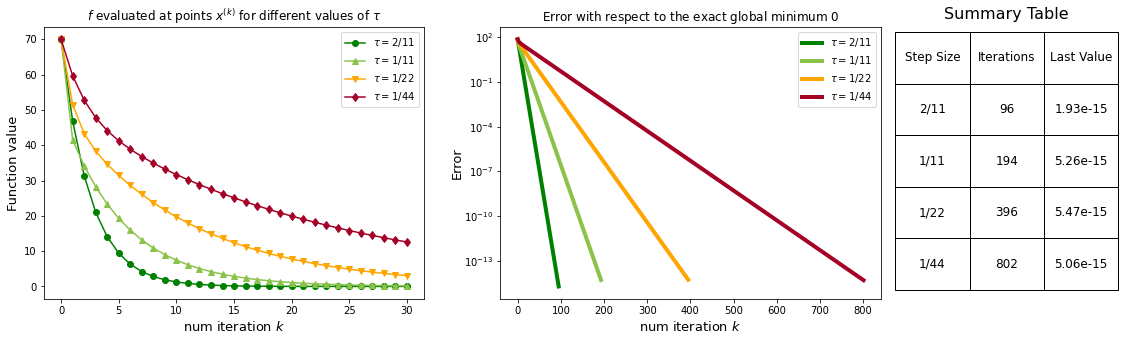
\includegraphics[width=1\textwidth]{Pictures/Merged_conv_ellipsoid_fixed_table.png}
    \caption{The left plot illustrates the convergence, while the middle plot shows the logarithmic error $f(x^{(k)})$ at each iteration up to the final iteration. On the right, a table summarizes the step sizes used, the total number of iterations, and the optimality gap.}\label{fig:convergence1_fixed}
\end{figure}\\
In order to visualize the convergence more effectively, contour plots can be very useful. A contour plot is a type of graph that shows how a function of two variables changes across different values. It does this by plotting contour lines, which are lines that connect points with the same value of the function. These contour lines help us visualize how the value of the function changes as we move around the graph. This can be particularly helpful for seeing how the gradient descent algorithm is moving towards the global minimum.
\newpage
The convergence can be visualized for different step sizes $\tau$. Let's choose $\tau_1 = 1/51$ and $\tau_2 = 2/11$. For step size $\tau_1$, gradient descent computes a minimizing sequence consisting of 930 vectors, and for $\tau_2$, as can be seen in the summary table in Figure \ref{fig:convergence1_fixed}, it computes a minimizing sequence consisting of 96 vectors. The contour plot below demonstrates the convergence for both step sizes by plotting the starting point $x^{(0)}=(10, 2),$ the two minimizing sequences and the contour lines of $f.$\footnote{See line~\ref{line:15} to~\ref{line:16} for the code to create the contour plot.}
\begin{figure}[h!]
    \centering
        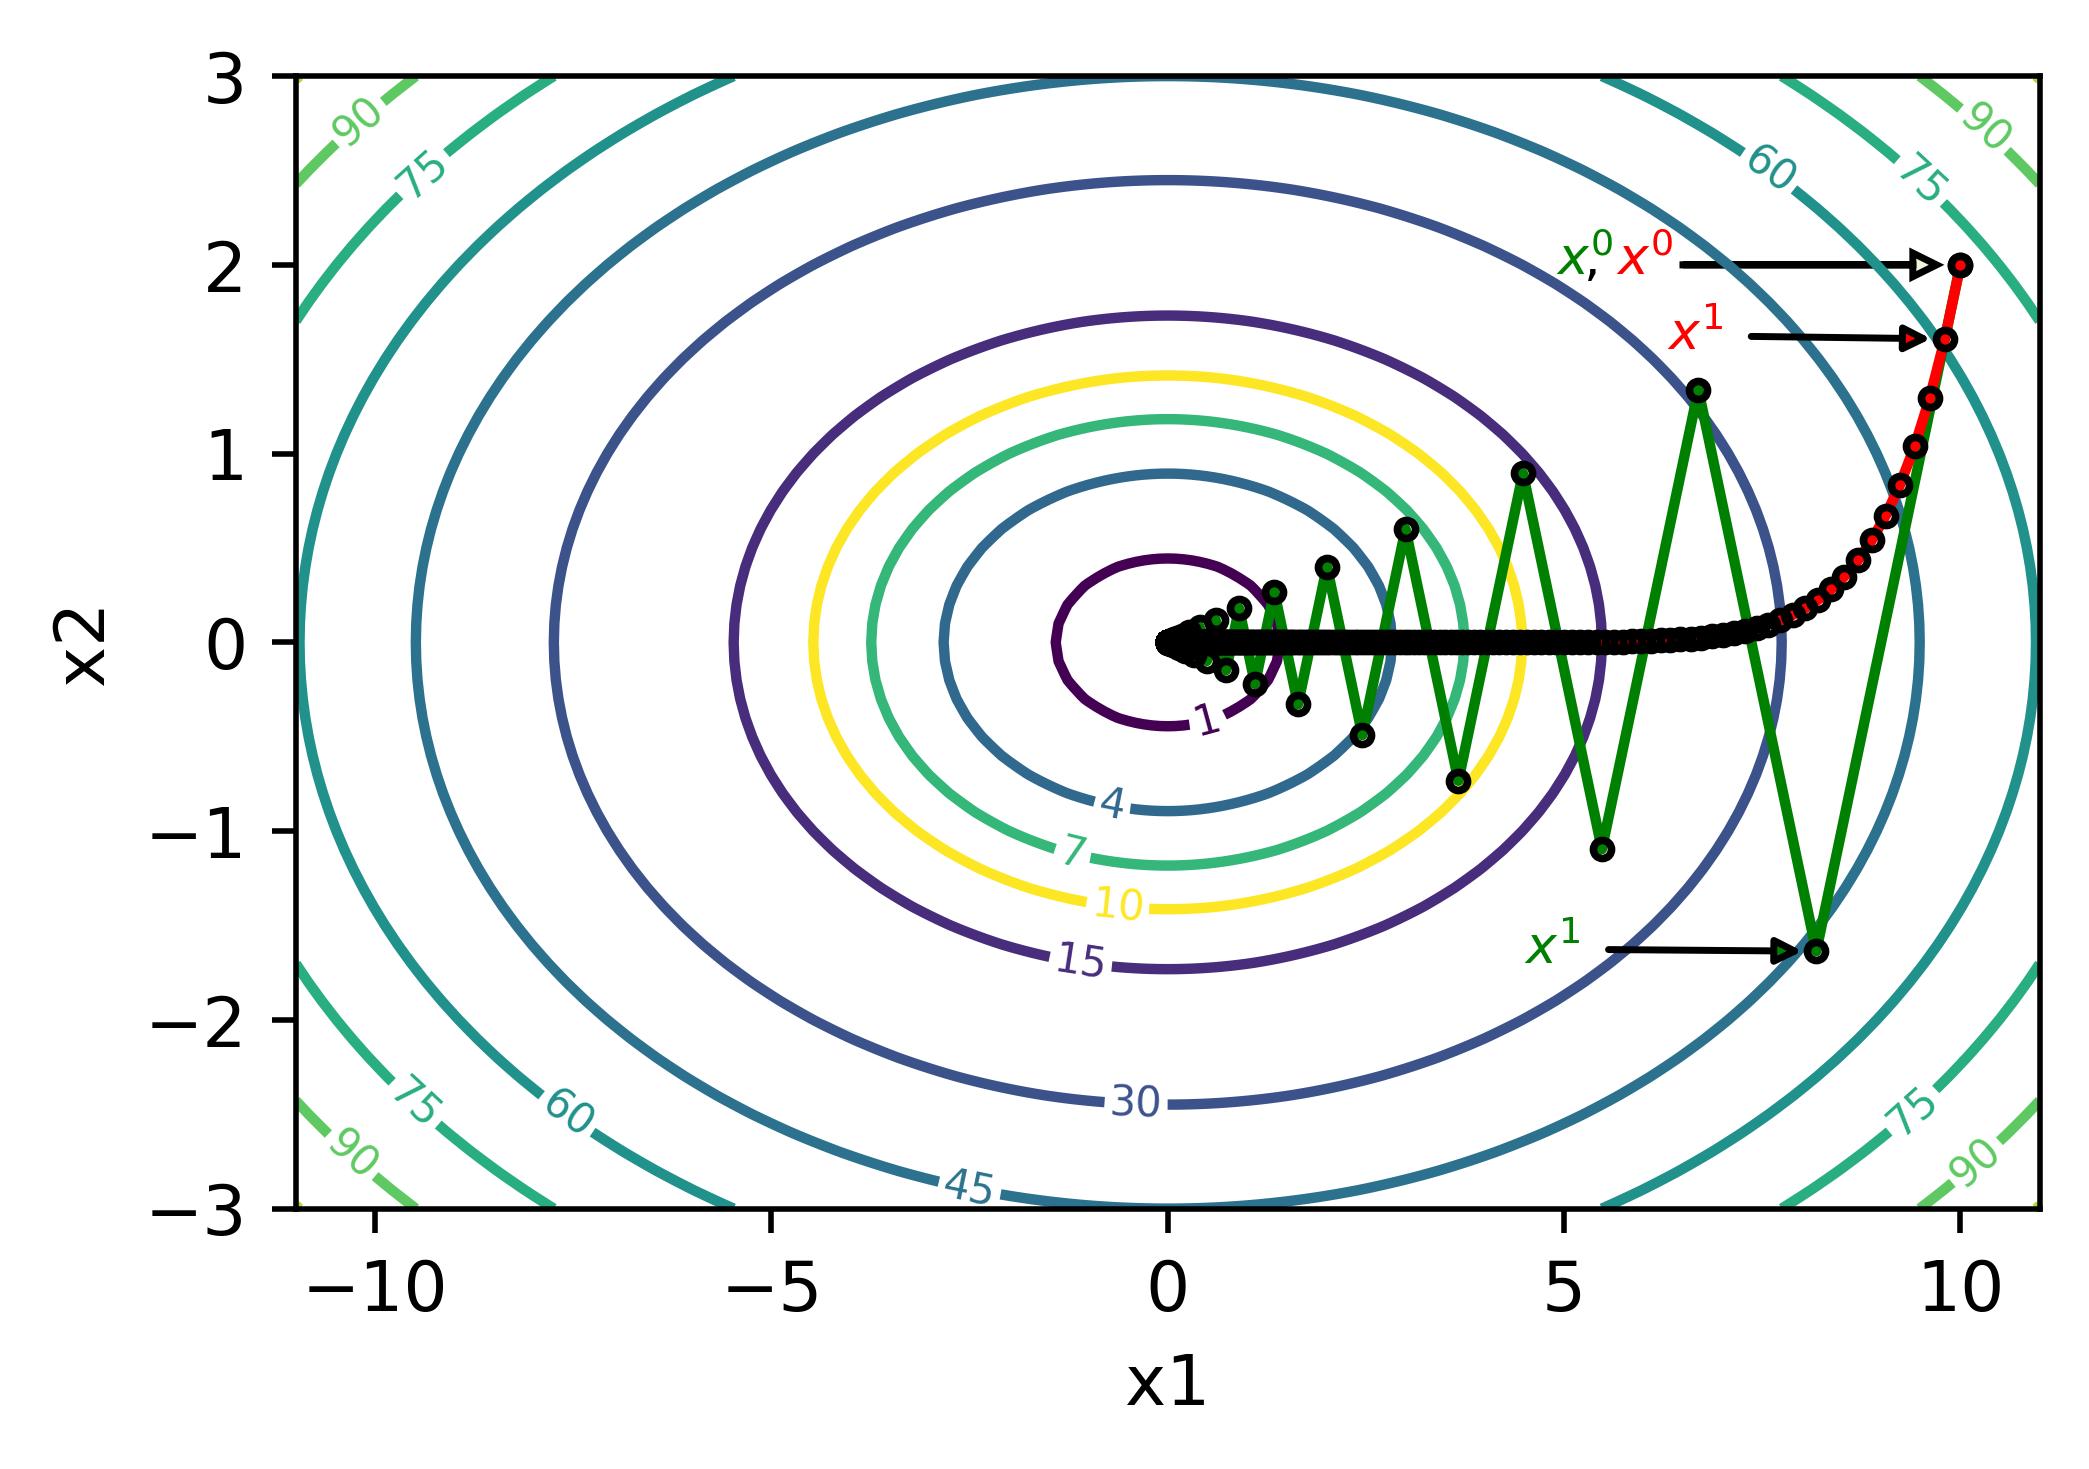
\includegraphics[width=0.65\textwidth]{Pictures/Level sets of ellipsoid_fixed.png}
    \caption{The color red represents the convergence with step size $\tau_{1}$ and green represents the convergence with step size $\tau_{2}.$ With step size $\tau_{2}$, the convergence is substantially faster than with step size $\tau_{1}.$ For sake of illustration $\tau_{1}$ was chosen to be compared to $\tau_{2}$, since $\tau_{1}$ satisfies the bound provided by \ref{pf_gd_sc_L}.}\label{fig:levelsets1_fixed}
\end{figure}\\
It is important to note that choosing a bound larger than $\tau_{2} = 2/11$ can cause some problems. In fact you can find yourself in unknown territory. Since if both $\tau \leq 2/(\alpha + L) $ and $\tau < 2\alpha / L^{2}$ are ignored, the likelihood that the algorithm diverges or overshoots the minimum, increases. The figure below shows the relation between the number of iterations until the algorithm terminates and the step size.\footnote{See line~\ref{line:17} to~\ref{line:18} for the code to create the plot.} 
\begin{figure}[h!]
    \centering
        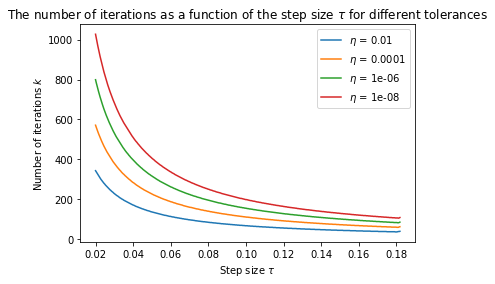
\includegraphics[width=0.75\textwidth]{Pictures/GD ellipsoid_fixed_iterations_vs_stepsize.png}
    \caption{As long as $\tau$ remains within the appropriate range, an increase in $\tau$ leads to faster convergence towards the global minimum, and hence a reduction in the number of iterations required for termination. Additionally, an increase in the tolerance $\eta$ results in faster convergence.}\label{fig:GD_ell_fixed_iter}
\end{figure}\\
\newpage
\subsubsection{Gradient descent with backtracking line search} Gradient descent using backtracking line search with $\alpha = 0.3$, $\beta = 0.8$ and $\eta = 10^{-7}$ is implemented on the quadratic function $f$.\footnote{See subsection \ref{GD-on-qd} for the implementation of GD with backtracking line search on $f.$} The number of iterations until the algorithm terminates is 92. So the algorithm computes a minimizing sequence that consists of 93 vectors: $(x^{(0)},\ldots,x^{(92)})$. The convergence of gradient descent to the exact global minimum $p^{*}=0$ with backtracking line search, can be visualized.\footnote{See line~\ref{line:p5} to~\ref{line:p6} for the code to create the convergence plots.} The optimality gap is the distance between $f(x^{(92)}) = 3.5\cdot 10^{-15}$ and $p^{*}=0$ which is precisely $f(x^{(92)}).$ In the following figure, on the left you can see an illustration of the convergence to $p^{*}=0$ and on the right the error $f(x^{(k)})$ with respect to $p^{*}=0$ for every $k$ up until 30.
\begin{figure}[h!]
    \centering
        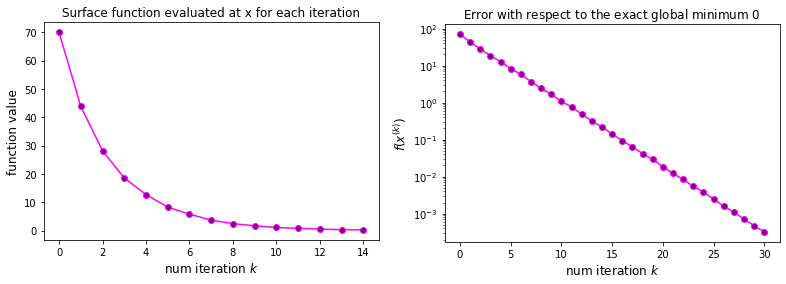
\includegraphics[width=0.85\textwidth]{Pictures/Merged_conv_ellipsoid.png}
    \label{fig:convergence1}
\end{figure}\\
The contour lines of the quadratic function $f$ and the points $(x^{(0)},\ldots,x^{(92)})$ are shown in the figure below.\footnote{See line~\ref{line:p7} to~\ref{line:p8} for the code to create the contour plot.}
\begin{figure}[h!]
    \centering
        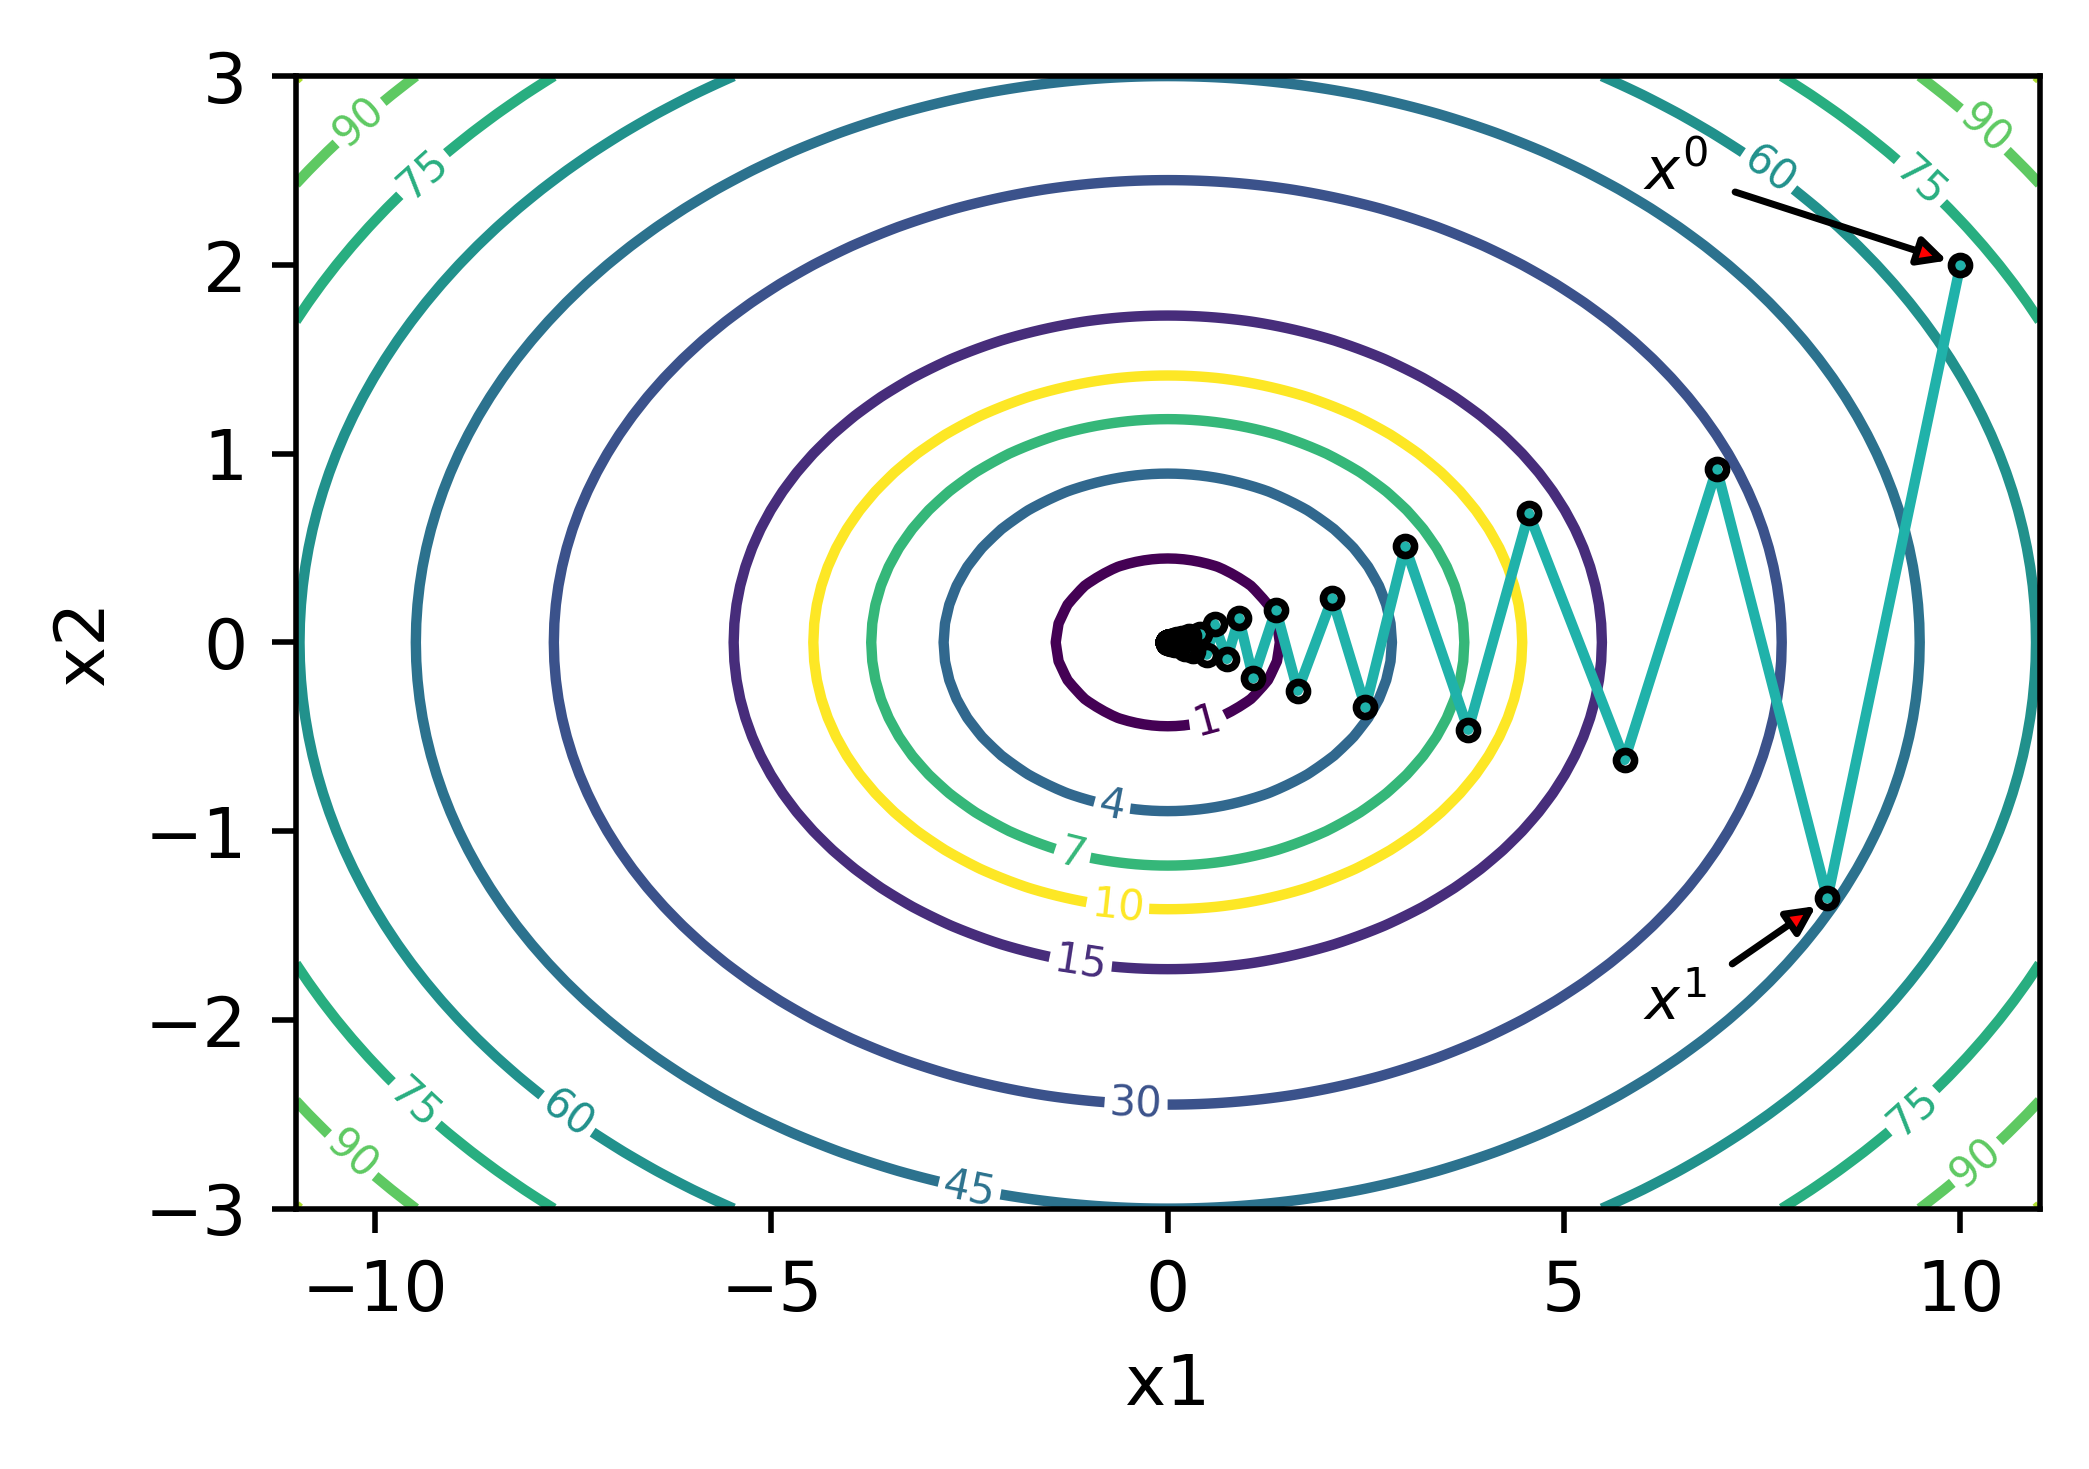
\includegraphics[width=0.58\textwidth]{Pictures/Level sets of ellipsoid.png}
    \label{fig:levelsets1}
\end{figure}
\newpage
\subsection{A non-quadratic problem}
We now consider a non-quadratic example in $\mathbf{R}^2$,  with 
\begin{equation*}\label{eq:12}\tag{5.2.1}
\begin{aligned}  
    &g(x) = e^{x_{1}+3x_{2}-0.1}+e^{x_{1}-3x_{2}-0.1}+e^{-x_{1}-0.1}
\end{aligned}
\end{equation*}
First it should be checked whether this function is convex. $g(x) = g_{1}(x)  + g_{2}(x) + g_{3}(x).$ Define: $f: y \mapsto e^{y}$. Then $g_{i}(x) = f(h_{i}(x)) \text{ } i=1,2,3$ and $g(x) = f(h_{1}(x)) + f(h_{2}(x)) + f(h_{3}(x)) ,$ where $h_{1}: x \mapsto x_{1} + 3x_{2}-0.1$, $h_{2}: x \mapsto x_{1} - 3x_{2}-0.1$, and $h_{3}: x \mapsto -x_{1}-0.1$. Since $f"(y) = e^{y} > 0 \text{ }$ for all $y \in \mathbf{R},$ $f$ is convex. Furthermore $h_{1}, h_{2}, h_{3}$ are affine. By definition \ref{compaf} the composition of a convex function with an affine function is convex, so $g_{i}(x) = f(h_{i}(x))$ is convex for $i=1,2,3.$ The sum of convex functions is also convex, therefore $g$ is convex. To get a visual impression, figure \ref{fig:exp} is a 3D plot of $g.$
\begin{figure}[h!]
    \centering
        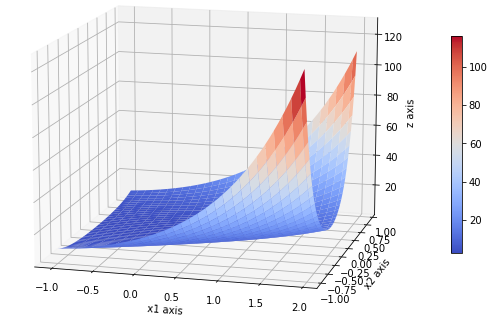
\includegraphics[width=0.36\textwidth]{Pictures/3D plot of an exponential function.png}
    \caption{3D surface plot of the function $g$}\label{fig:exp}
\end{figure}\\
Gradient descent using backtracking line search with $\alpha = 0.1$, $\beta = 0.7$ and stopping criterion $\eta = 10^{-7}.$ is implemented on the non-quadratic function $g$.\footnote{See subsection \ref{GD-on-nqd} for implementation of GD with backtracking line search on $g$.} The starting vector is chosen to be $x^{(0)} = (-1,0.5)$. The algorithm computes a minimizing sequence of 39 vectors. Together with the starting point we find the sequence: $(x^{(0)},\ldots,x^{(39)}).$ The function value decreases iteration after iteration and whenever $||\nabla f(x)||_{2} \leq \eta$, the algorithm terminates. The figure below shows the convergence to the global minimum $p^{*} \approx g(x^{(39)})=2.559$, where the plot on the left is an illustration of the convergence to $p^{*}$ and the one on the right the error $g(x^{(k)}) - g(x^{(39)})$ for every k up until 39.\footnote{See line~\ref{line:p9} to~\ref{line:p10} for the code to create the convergence plots.} 
\begin{figure}[h!]
    \centering
        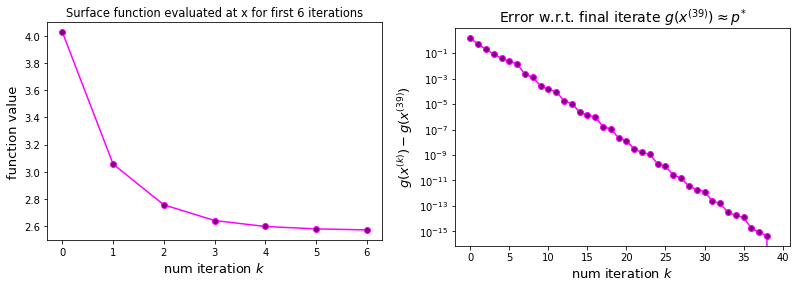
\includegraphics[width=0.72\textwidth]{Pictures/Merged_conv_exponential.png}
    \label{fig:convergence2}
\end{figure}\\
Similarly to the the quadratic function, it is possible to provide a contour plot for $g.$ The contour lines of the non-quadratic function $g$ and the points $(x^{(0)},\ldots,x^{(39)})$ are shown in the figure below.\footnote{See line~\ref{line:p11} to~\ref{line:p12} for the code to create the contour plot.}
\begin{figure}[h!]
    \centering
        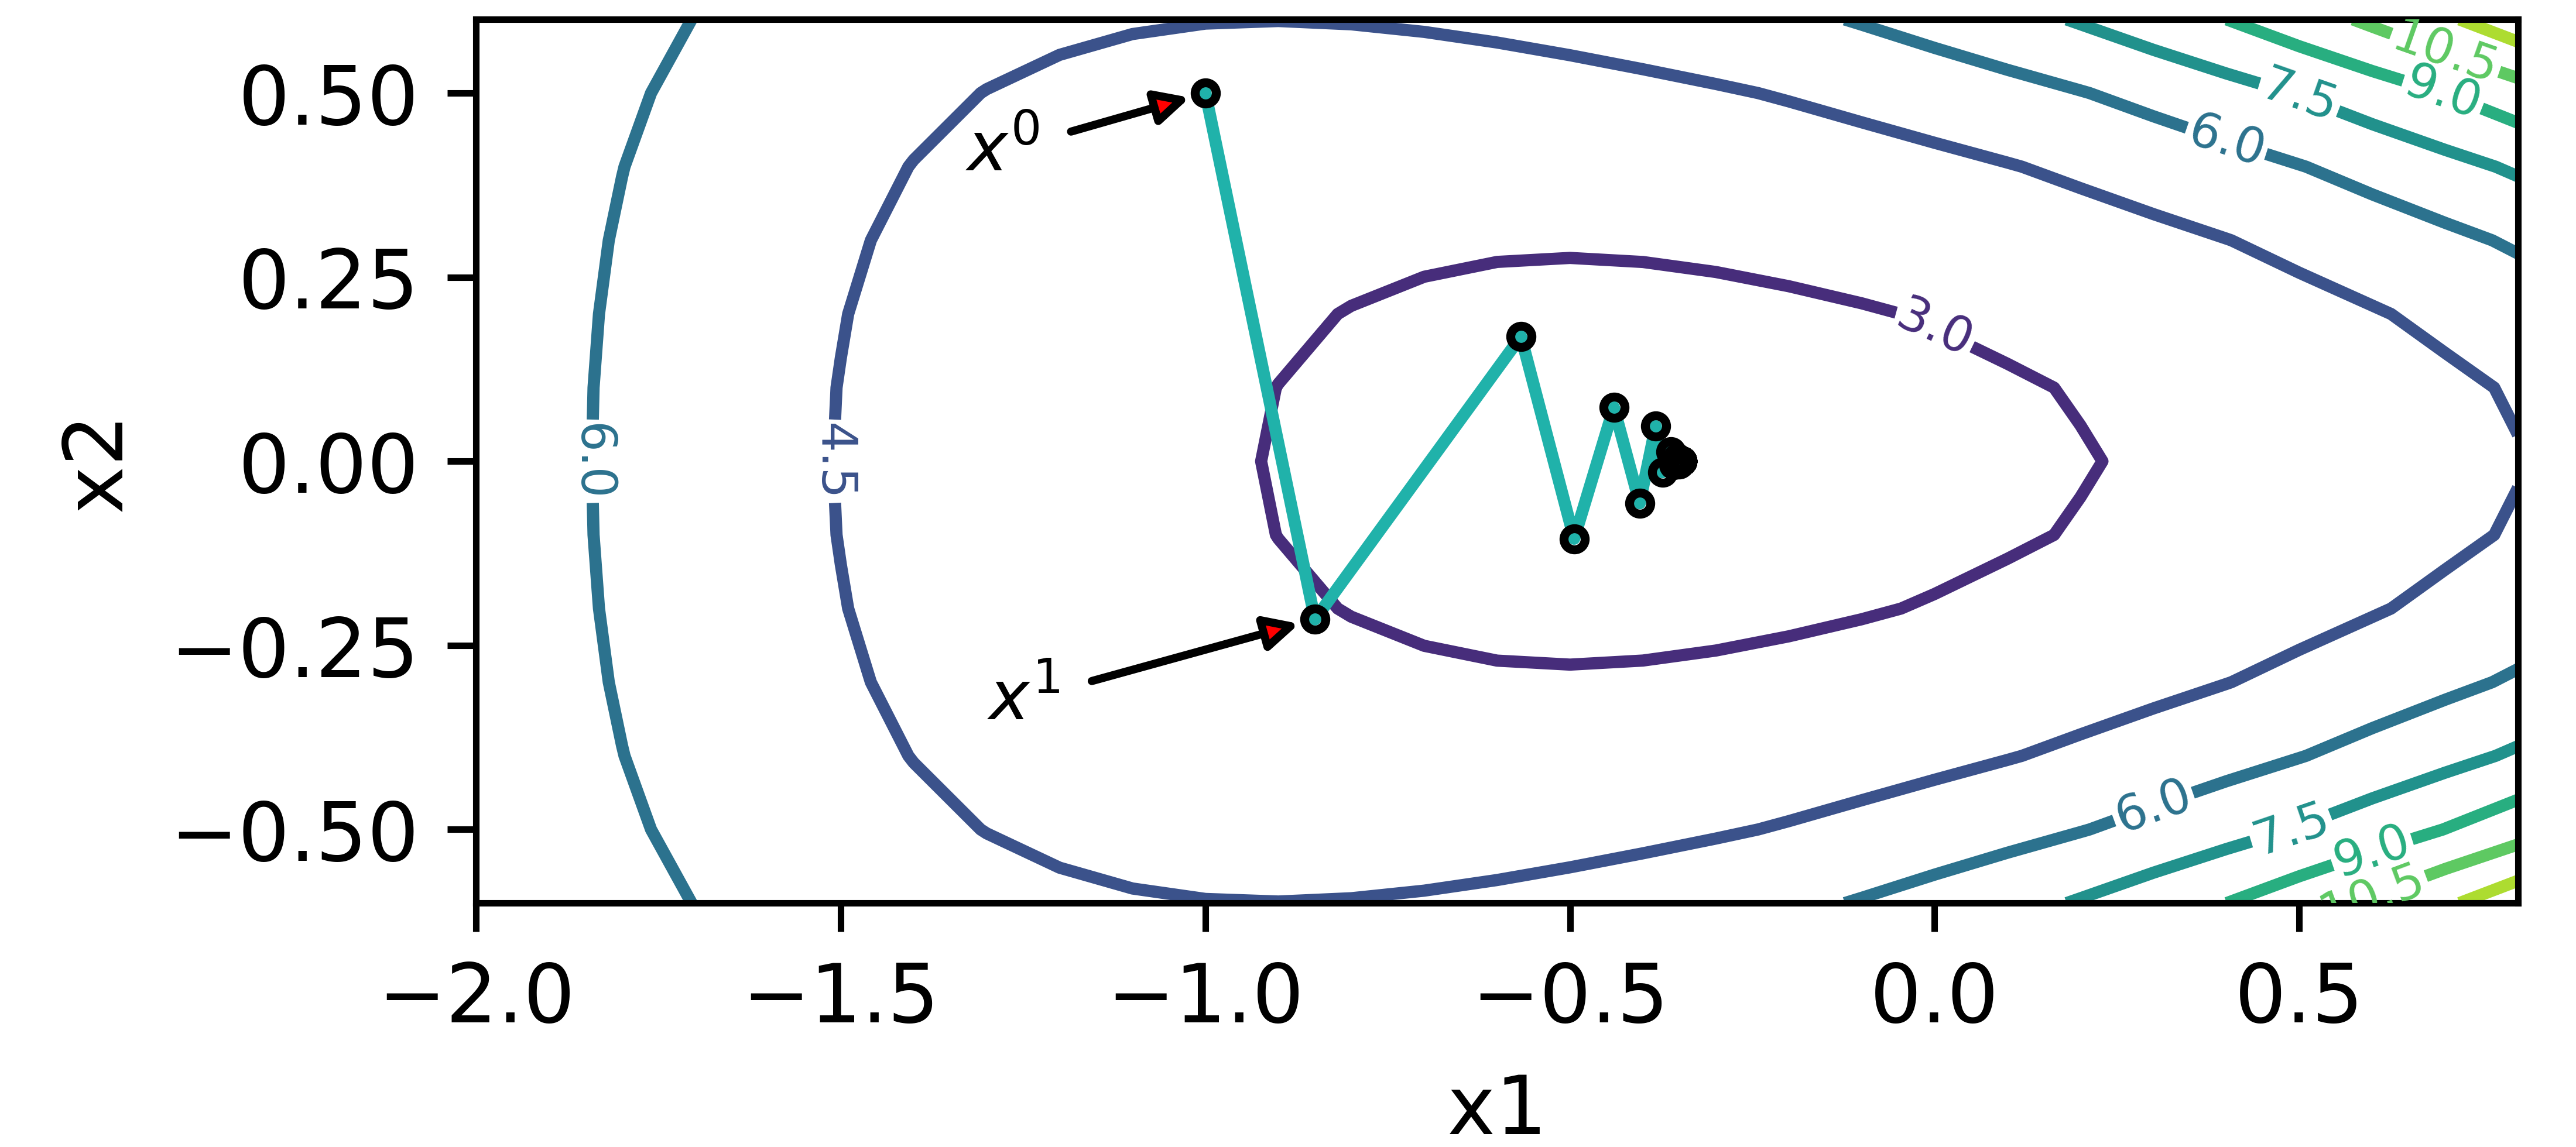
\includegraphics[width=0.55\textwidth]{Pictures/Level sets of exponential.png}
    \label{fig:levelsets2}
\end{figure}\\
\newpage
\subsection{A multi-dimensional non-convex problem}
The function that will be considered is Ackley's function.\ref{eq:18} This function is widely used for testing optimization algorithms.\cite{Test_functions} In its two-dimensional form, as shown in \ref{fig:Ackelys_plot}, it is characterized by a nearly flat outer region, and a large hole at the centre.\footnote{See line~\ref{line:19} to~\ref{line:20} for the code to create 3D plots of Ackley's function.}
\begin{equation*}\label{eq:18}\tag{5.3.1}
\begin{aligned}
&h(x) = -a\exp\left(-b\sqrt{\frac{1}{d}\sum_{i=1}^{d} x_{i}^{2}}\right) - \exp\left(\frac{1}{d}\sum_{i=1}^{d} \cos(cx_{i})\right) + a + \exp(1) 
\end{aligned}
\end{equation*}
\begin{figure}[h!]
    \centering
        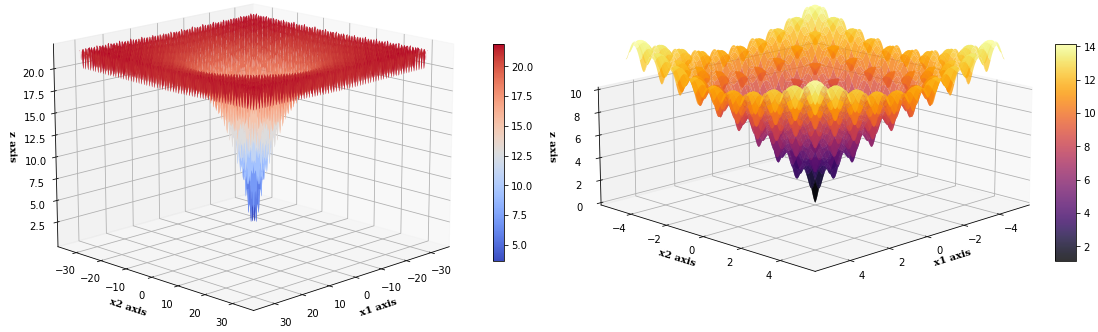
\includegraphics[width=0.85\textwidth]{Pictures/Merged_Ackleys_plot.png}
    \caption{3D plots of $h$ on $x_{i} \in [-32.768,\text{ } 32.768]$, and on $x_{i} \in [-5,\text{ } 5]$}\label{fig:Ackelys_plot}
\end{figure}\\
 Many loss functions in machine learning are non-convex. $h$ is an example of a non-convex function that is multimodal, i.e., it has multiple local minima. This possesses a risk for gradient-based optimization methods, since they can become trapped in one of the local minima and thus fail to find the global minimum. Therefore, it is a good benchmark function to evaluate the performance of gradient-based optimization methods. The global minimum of $h$ is known, namely when $x^{*} = \vec{0}$ , $h(x^{*}) = 0.$ 
 \subsubsection{Gradient descent with backtracking line search}
 Consider $h$ with dimension $d=100.$ For the variable values take: $a = 20,\text{ }b = 0.2,$ and $c = 2\pi$. Gradient descent using backtracking line search with $\alpha = 0.1, \beta = 0.8$ and stopping criterion $\eta = 1e-6$ is implemented on $h.$\footnote{See subsection \ref{GD-Ack} for implementation of GD with backtracking line search on $h.$} To test convergence, a vector $x^{(0)}$ is created randomly such that each term lies in $[-32.768, 32.768]$.\footnote{See \ref{line:21} for the code to create a random vector.} Secondly, the algorithm is tested by choosing a starting vector that is close to the origin, namely $x^{(0)}=(0.4,\ldots,0.4).$ Figure \ref{fig:Ackelys_conv_check} shows the progression of the algorithm for the two different starting vectors.\footnote{See line~\ref{line:22} to~\ref{line:23} for the code to create the convergence plots.}
\begin{figure}[h!]
    \centering
        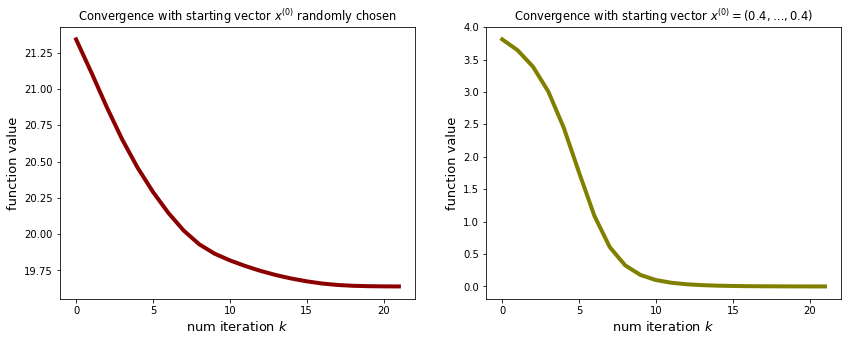
\includegraphics[width=0.75\textwidth]{Pictures/Merged_conv_ackleys.png}
    \caption{Plots to check convergence of GD for two different starting vectors.}\label{fig:Ackelys_conv_check}
\end{figure}\\
\newpage
From the results in Figure \ref{fig:Ackelys_conv_check}, the main limitation of gradient descent becomes evident: it is highly susceptible to local minima due to its inherent reliance on gradient information. For a randomly created starting vector, the algorithm converges towards one of the many local minima of $h$, and only if $x^{0}$ is chosen to be very close to the optimal solution, it achieves convergence towards the global minimum. This experiment underscores the importance of selecting appropriate optimization methods for specific problems. A natural question that arises is whether stochastic gradient descent (SGD) can be applied to this problem. SGD is specifically designed for objective functions that arise in machine learning and deep learning, which typically involve large datasets. However, $h$ is a mathematical optimization problem that does not have the desirable form of a sum of functions. Consequently, there is no natural way to divide the function into smaller subsets. In other words, the gradient information in $h$ is deterministic and does not depend on a dataset, which eliminates stochasticity from the problem and makes SGD less applicable.

\subsubsection{Simulated Annealing}
An alternative to gradient descent is simulated annealing with pseudo-code given in \ref{Pseudocode_SA}. The problem parameters remain unchanged: $d=100, a=20, b=0.2,$ and $c=2\pi.$ The algorithm is tested for two different starting vectors, namely one that is randomly generated with terms lying in $\left[-32.768,32.768\right]$ and one that is closer to the optimal solution with terms in $\left[-5,5\right].$ The initial temperature is chosen to be $t_0=5.0$ and cooling schedule $t_{k} = 0.99^{k}t_0.$ The algorithm terminates when the maximum number of iterations $k_{max}=400$ is reached. The figures \ref{fig:SA_conv1} and \ref{fig:SA_conv2} below depict the possible paths the algorithm can take to progress towards the global minimum of $h$. In the left figure, the algorithm converges for both starting vectors, whereas the right figure shows a scenario in which the algorithm for one of the starting vectors gets trapped in a local minimum of $h$. 

\begin{figure}[h]
  \centering
  \begin{minipage}[b]{0.3687\textwidth}
    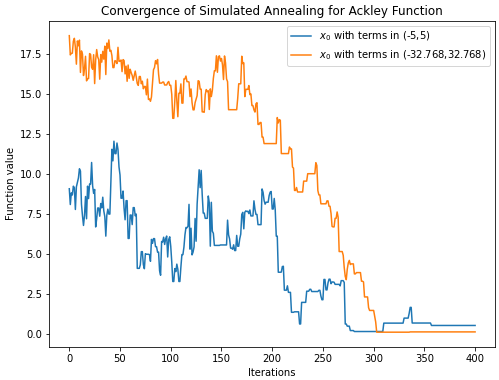
\includegraphics[width=\textwidth]{Pictures/sa_convergence-ackley3-38-c.png}
    \caption{Example 1}\label{fig:SA_conv1}
  \end{minipage}
  \hspace{0.05cm} 
  \begin{minipage}[b]{0.36\textwidth}
    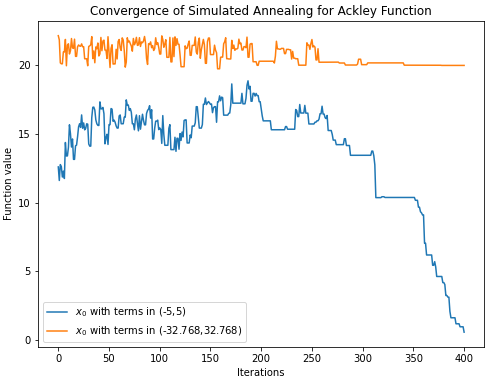
\includegraphics[width=\textwidth]{Pictures/sa_convergence-ackley3-37_c.png}
    \caption{Example 2}\label{fig:SA_conv2}
  \end{minipage}
\end{figure}
In order to visualize the stochasticity in the algorithm, $h$ with dimension $d=2$ is considered. In this setting, contour plots of $h$ and the progression of simulated annealing towards possibly the global minimum can be plotted. The figures \ref{fig:SA_cont1} and \ref{fig:SA_cont2} below depict the progression of two different starting vectors in $\mathbf{R}^2$ with terms in $\left[-10, 10\right]$ towards the global minimum.
\begin{figure}[h]
    \centering
    \begin{minipage}[b][0.38\textwidth]{0.35\textwidth}
      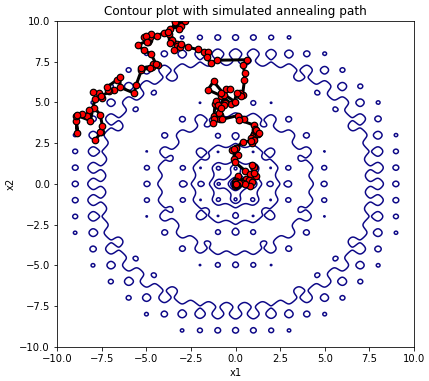
\includegraphics[width=\textwidth]{Pictures/sa_convergence-ackley_contour11.png}
      \caption{Example 1}\label{fig:SA_cont1}
    \end{minipage}
    \hspace{0.05cm}
    \begin{minipage}[b][0.38\textwidth]{0.35\textwidth}
      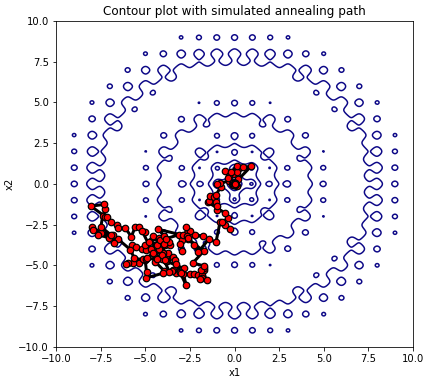
\includegraphics[width=\textwidth]{Pictures/sa_convergence-ackley_contour18.png}
      \caption{Example 2}\label{fig:SA_cont2}
    \end{minipage}
\end{figure}
\subsubsection{Particle Swarm Optimization (PSO)}
As described in Section \ref{PSO_s}, Particle Swarm Optimization (PSO) is a stochastic global optimization algorithm that performs well on multi-dimensional non-convex functions. As such, it is worth applying to minimize $h$. The algorithm is implemented in Python with cognitive and social constants set to $C_{1}=0.5$ and $C_{2}=0.3$, respectively, and the maximum number of iterations is set to $k_{max}=2000$. The only remaining parameter to determine is the size of the swarm. It is insightful to visualize the trajectory of the best function evaluations (i.e., the lowest function values in each iteration) up until termination for different swarm sizes. The following figure displays the trajectories for various swarm sizes, specifically for $N=50$, $N=200$, $N=500$, and $N=1000$. The table on the right provides the best cost (lowest function evaluation) for each of the four swarm sizes. The results are presented below (Figure \ref{fig:PSOConvMultipleSwarmSizes}).
\begin{figure}[h!]
    \centering
        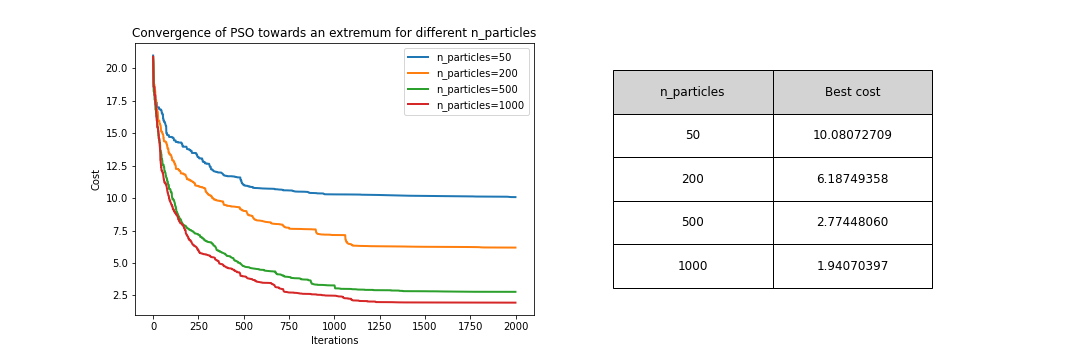
\includegraphics[width=1.12\textwidth]{Pictures/PSO_convergence-ackley_multiple_n_particles_with_table.png}
    \caption{This figure displays four trajectories of PSO distinguished by different swarm sizes n$\textunderscore$particles on the left and the best cost obtained for each of the cases in a table on the right.}\label{fig:PSOConvMultipleSwarmSizes}
\end{figure}\\
As can be seen from the figure, an increase in the swarm size, leads to convergence towards a minimum with a lower cost. It can also be noted, that none of the four cases reach the global minimum. This has to do with the design of the algorithm. PSO does not allow for worse function values (i.e., ones that are higher than the previous iterations), therefore it is sensitive to getting stuck in local minima. $h$ contains many local minima, and some of these local minima are very close to the global minimum. The number of local minima increases when the dimensionality of the problem increases. Since in this example, the dimension is $d=100,$ it becomes very unlikely for the swarm to collectively reach the global minimum. When $d$ is kept low, the likelihood that the algorithm succeeds in reaching the global minimum increases. To see whether this is indeed the case, PSO is performed on $h$ with $d=2.$ $C_{1}$ and $C_{2}$ remain unchanged. $k_{max}$ is set to $100$ and the size of the swarm is set to $50.$ The following figure shows the trajectory of the swarm towards the global minimum. Three different time steps are taken, namely $k=0,$ $k=10,$ and $k=100.$ For each time step a contour plot of the function and the positions of the particles are depicted in figure (Figure \ref{fig:PSO_2D_swarm}) below.
\begin{figure}[h!]
    \centering
        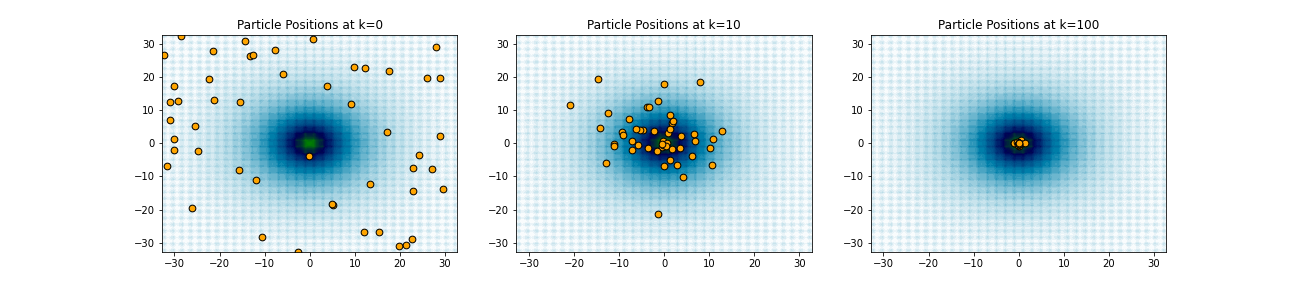
\includegraphics[width=1\textwidth]{Pictures/PSO_ackleys_2D_swarm.png}
    \caption{Contour plots and particle positions at time steps $k=0,$ $k=10,$ and $k=100$}\label{fig:PSO_2D_swarm}
\end{figure}\\
\newpage
\subsubsection{Comparison of Methods}
The effectiveness of various optimization methods was compared in minimizing Ackley's function $h$. First, gradient descent with backtracking line search was implemented. Before the implementation, it was anticipated that the algorithm's likelihood of finding the global minimum would be low. This is because Ackley's function contains numerous local minima that are closely spaced, and since gradient descent is highly sensitive to extrema, it can easily get stuck in a local minimum that isn't the global minimum. The results support this notion, as the algorithm became stuck in a local minimum when starting from a random vector. Next, simulated annealing (SA) was implemented and found to perform quite well. In fact, it was able to locate the global minimum. The primary reason for this success is that the algorithm is designed to escape local minima easily by allowing hill-climbing moves, which temporarily worsen the function evaluation outcome. Finally, particle swarm optimization (PSO) was implemented. This algorithm performed better than gradient descent by finding superior solutions, but it was still outperformed by SA, as it could not locate the global minimum. Additionally, to obtain a better solution with PSO, the swarm size had to be significantly increased, which greatly impacted computation time. In conclusion, both SA and PSO performed better than gradient descent. However, it is important to note that these algorithms were more computationally expensive, as their execution required more time than gradient descent.

\subsection{Application of SGD on a Neural Network}
\subsubsection{The Data}
In the realm of optimization, Stochastic Gradient Descent (SGD) is often applied to suitable functions associated with feed-forward neural networks. These networks are chosen because the objective functions that they generate typically take the form of a large sum of smaller functions. In each iteration of SGD, the gradient of one of these smaller functions, $\nabla f_{i(k)}(x_{k})$ where $i(k)$ is drawn uniformly at random from $\{1,\ldots,n\}$, is computed. Here, $n$ denotes the size of the dataset, i.e., the total number of training examples. This gradient serves as an unbiased estimator of the true gradient of the cost function. By applying the SGD update formula, an optimal solution can be found. For this application, the MNIST dataset of handwritten digits will be considered \cite{deng2012mnist}. This dataset is a common choice in the field of neural networks due to its simplicity. Each data point in the MNIST dataset is a pair comprising a grayscale handwritten image of a digit (28 pixels by 28 pixels) and its associated label indicating the true value of the digit. The dataset contains $n=60,000$ such data pairs. To prepare the images for input into the neural network, the 28x28 pixel image is flattened into a 1D array of 784 elements. Each element represents a grayscale value between 0 (black) and 255 (white), which are typically normalized to be a floating-point number between 0 and 1. Thus, an example input vector for the neural network is $x^{(i)} \in \mathbf{R}^{784}$, where $i \in \{1,\ldots,n\}.$ The output vector $\hat{y}^{(i)} \in \mathbf{R}^{10}$, where $i \in \{1,\ldots,n\}$, can be interpreted as a probability distribution over the ten digit classes, 0-9. Each component of the vector, $\hat{y_{j}}^{(i)}$, where $j \in \{1,\ldots,10\}$, represents the predicted probability that the input image corresponds to the digit class $j-1$. Hence, the sum of all the entries in $\hat{y}^{(i)}$ is 1, conforming to the properties of a probability distribution. For instance, if all the entries in the vector $\hat{y}^{(i)}$ are equal to 0.1, it would imply that the network is uncertain about the digit class of the input image, assigning an equal probability to each class. Ideally, during training, the neural network learns to confidently classify each image into one of the 10 classes, representing the digits 0-9. This means that the output vector $\hat{y}^{(i)}$ should have one entry that is significantly larger than the others, indicating a high probability for a particular digit class.

\subsubsection{Neural Network Architecture}
The neural network architecture is defined in the programming language Python \cite{python} using the open-source deep learning framework PyTorch \cite{NEURIPS2019_9015}. The neural network here is a feed-forward neural network consisting of an input layer, two hidden layers and an output layer. The input layer consists of 784 neurons, which is the size of the flattened input image. This layer is fully connected to the first hidden layer consisting of 128 neurons. This hidden layer is fully connected to the next hidden layer consisting of 64 neurons. This final hidden layer is fully connected to the output layer consisting of 10 neurons. So, the structure of the network is: Input(784) - Hidden1(128) - Hidden2(64) - Output(10).

\subsubsection{Training Procedure}
\begin{comment}
The training data of handwritten digits $x^{(1)},\ldots,x^{(n)},$ where $n=60000$ is the size of the dataset, is randomly shuffled and divided into mini-batches with each mini-batch consisting of $\approx 64$ examples. For each mini-batch each of the 64 input vectors are forward passed through the network. The 784 neurons in the input layer are connected to each of the 128 neurons in the first hidden layer. The first set weights and biases is initialized. This set consists of $784\cdot128 = 100,352$ weights and 128 bias terms. In each neuron in the first hidden layer, the dot product between the input vector $x$ and $w$ is computed and one bias term is added to the result yielding $w^{T}x + b_{1}.$ Then the ReLU (Rectified Linear Unit) activation function which is defined as: ReLu$(x) = \max{0, x}$, is applied on $w^{T}x + b_{1},$ and ReLU$(w^{T}x + b_{1})$ is computed. This procedure is done The training data of handwritten digits, $x^{(1)},\ldots,x^{(n)},$ with $n=60000$ being the size of the dataset, is randomly shuffled and divided into mini-batches. Each mini-batch consists of roughly 64 examples. For each mini-batch, we have a matrix of input vectors $X \in \mathbb{R}^{m \times 784}$, where $m$ is the batch size (~64), and each row of $X$ is an input vector $x^{(i)}$. The 784 neurons in the input layer are connected to each of the 128 neurons in the first hidden layer. The weights connecting these layers are represented by a matrix $W^{(1)} \in \mathbb{R}^{784 \times 128}$, and the biases for the first hidden layer as a vector $b^{(1)} \in \mathbb{R}^{128}$. These parameters are initialized before the training process starts. In each neuron in the first hidden layer, a linear transformation of the form $XW^{(1)} + b^{(1)}$ is computed. Here, $W^{(1)^T}x^{(i)} + b^{(1)}$ represents the dot product between each input vector and the corresponding column of $W^{(1)}$, with the bias term added. The ReLU (Rectified Linear Unit) activation function is then applied element-wise on this output, yielding $H^{(1)} = \text{ReLU}(XW^{(1)} + b^{(1)})$. The matrix $H^{(1)} \in \mathbb{R}^{m \times 128}$ stores the outputs of the first hidden layer, where each row corresponds to the output for a specific input vector from the mini-batch.
This procedure is repeated for the second hidden layer, now using $H^{(1)}$ as the input and applying weights $W^{(2)} \in \mathbb{R}^{128 \times 64}$ and biases $b^{(2)} \in \mathbb{R}^{64}$. Thus, we compute $H^{(2)} = \text{ReLU}(H^{(1)}W^{(2)} + b^{(2)})$. Finally, the output layer of the network performs another linear transformation on the output of the second hidden layer. This yields the output vector $\hat{Y} = H^{(2)}W^{(3)} + b^{(3)}$, where $\hat{Y} \in \mathbb{R}^{m \times 10}$ and each row corresponds to the network's prediction for a specific input digit.
\end{comment}
The training data of handwritten digits, $\{x^{(1)},\ldots,x^{(n)}\},$ with $n=60000$ being the size of the dataset, is randomly shuffled and divided into mini-batches. Each mini-batch consists of roughly 64 examples. For each mini-batch, we have a matrix of input vectors $X \in \mathbb{R}^{m \times 784}$, where $m$ is the batch size ($\approx64$), and each row of $X$ is an input vector $x^{(i)}$.

The 784 neurons in the input layer are connected to each of the 128 neurons in the first hidden layer. The weights connecting these layers are represented by a matrix $W^{(1)} \in \mathbb{R}^{784 \times 128}$, and the biases for the first hidden layer as a vector $b^{(1)} \in \mathbb{R}^{128}$. These parameters are initialized before the training process starts.

In each neuron in the first hidden layer, a linear transformation of the form $XW^{(1)} + b^{(1)}$ is computed. Here, $W^{(1)^T}x^{(i)} + b^{(1)}$ represents the dot product between each input vector and the corresponding column of $W^{(1)}$, with the bias term added. The ReLU (Rectified Linear Unit) activation function is then applied element-wise on this output, yielding $H^{(1)} = \text{ReLU}(XW^{(1)} + b^{(1)})$.

The matrix $H^{(1)} \in \mathbb{R}^{m \times 128}$ stores the outputs of the first hidden layer, where each row corresponds to the output for a specific input vector from the mini-batch.

This procedure is repeated for the second hidden layer, now using $H^{(1)}$ as the input and applying weights $W^{(2)} \in \mathbb{R}^{128 \times 64}$ and biases $b^{(2)} \in \mathbb{R}^{64}$. Thus, we compute $H^{(2)} = \text{ReLU}(H^{(1)}W^{(2)} + b^{(2)})$.

Finally, the output layer of the network performs another linear transformation on the output of the second hidden layer. This yields the output vector $\hat{Y} = H^{(2)}W^{(3)} + b^{(3)}$, where $\hat{Y} \in \mathbb{R}^{m \times 10}$ and each row corresponds to the network's prediction for a specific input digit.














-
\clearpage\section{Conclusion and Future Work}
\paragraph{Summary of Results}
The main goal of this thesis was to explore deterministic and stochastic schemes for solving unconstrained optimization problems. One of the methods discussed was batch gradient descent (BGD), which proved to be especially useful for minimizing convex functions. From the convergence analysis of BGD with a fixed step size, it was found that for $\alpha$-strongly convex and $L$-smooth functions, the step size $\tau$ should be chosen to be approximately $\max\{2\alpha/L^{2}, \text{ } 2/(\alpha + L)\}.$ When the function was not strongly convex or when it was difficult to determine its convexity, it was determined that the step size should be chosen to be at most $\tau=1/L.$ In this case, BGD yielded a slower running time of $O(1/k)$. However, when the strong convexity assumption was present, BGD's running time was faster, at $O(C^{k}),$ where $C\in(0,1)$. Both BGD with a fixed step size and BGD with backtracking line search were applied to a quadratic strongly convex function. We found that the variant using line search outperformed the one with a fixed step size, albeit not by a significant margin. It was also revealed that BGD could be applied to non-convex functions. However, due to its reliance on gradient information, it can easily become trapped in a local minimum, thus failing to locate a global minimum. This study primarily focused on understanding and implementing a stochastic variant of gradient descent, known as Stochastic Gradient Descent (SGD). SGD is specifically designed to minimize large-scale non-convex cost functions that arise in machine learning. Given the gradient-based nature of SGD, like BGD, it is susceptible to getting stuck in local minima. In this study, this was observed to be a potentially beneficial property for machine learning models, as in many cases, a good local minimum can provide a satisfactory solution.  Moreover, a model that achieves the global minimum on training data might not generalize well to new data due to overfitting, whereas a local minimum could strike a better balance between fitting the data and generalizing to new examples as discussed in \cite[282-290]{Goodfellow-et-al-2016}. In machine learning, SGD often outperforms BGD for non-convex cost functions. This is because SGD can escape shallow local minima, while BGD tends to get stuck in the first local minimum it encounters. Furthermore, if the size of the training dataset $n$ is too large, it is impractical to compute the full gradient at each iteration. Then SGD is favored over BGD regardless of the function's convexity. The only time that BGD is preferred over SGD is when dealing with a not-too-large dataset and a convex cost function. In this study, SGD was applied to the Mean Squared Error (MSE) cost function given in Equation \eqref{MSE_cost_fun}. This function was computed based on labeled data of handwritten digits and outputs from a deep neural network designed to predict the labels of these digits. By employing SGD on the MSE cost function, a more optimal set of parameters was determined, which improved the neural network's ability in classifying the handwritten digits. It is noteworthy that SGD is suitable for cost functions in machine learning, as they typically take the form of a sum of functions. However, many non-convex functions like Ackley's function, given in equation \eqref{eq:18}, cannot be written as a sum of functions. In these situations, BGD outperforms SGD, simply because SGD isn't applicable. Global optimization methods become the preferred choice for non-convex functions like Ackley's function, where gradient-based methods aren't effective. Unlike gradient-based methods, these approaches, such as Simulated Annealing (SA) and Particle Swarm Optimization (PSO), employ diverse search strategies to thoroughly explore the solution space. This increases the likelihood of identifying the global minimum, as detailed in \cite[1-5]{horst1995handbook}. In machine learning, these methods are often not preferred over SGD due to their relatively slower convergence compared to SGD.
\paragraph{Future Work}
This thesis has offered insights into various optimization techniques. Some of these techniques, like BGD, are regarded as classical approaches, while others, such as SGD, are considered innovative. This study opens several avenues for exploration. For example, one can investigate different variants of BGD. One possible variant to study is called Gradient Descent with Momentum. This method uses a momentum term in the update process, which could potentially accelerate convergence. Additionally, one can explore adaptive gradient descent algorithms like AdaGrad, RMSProp and Adam. These methods dynamically adjust the step size, which could speed up convergence. Extending these algorithms to their stochastic versions could result in SGD variants worth investigating. This study explored unconstrained optimization problems. However, it is also possible to investigate constrained problems and explore the applicability of gradient descent methods in such scenarios. Furthermore, conducting a comparative analysis of SA and PSO on a wider range of benchmark functions could be effective in understanding their respective strengths and weaknesses. Additionally, exploring the application of SA and PSO in real world-scenarios across domains such as engineering, finance, or machine learning could reveal their effectiveness for solving practical optimization tasks.

\appendix
\titleformat{\section}{\normalfont\Large\bfseries}{}{0pt}{Appendix}
\clearpage\section{Appendix: Theorems}
\begin{theorem}\label{spectral norm}
\textnormal{\cite[3]{matrixnorms}}
The matrix norm induced by the vector norm $||\cdot||_{2}$ can be expressed, for an $n\times n$ matrix $A = (a_{ij})_{1\leq i,j \leq n} \in \mathbb{R}^{n\times n},$ as $$||A||_{2}=\sqrt{\underset{1 \leq i \leq n}{\max}\lambda_{i}},$$
where $\lambda_{i},\text{ }i=1,\ldots,n$ are the \textnormal{eigenvalues} of the matrix $A^{T}A.$
\end{theorem}
\begin{proof}
    The proof for this theorem is not included here as it doesn't significantly contribute to the central theme of this thesis. The interested reader may refer to \cite[4]{matrixnorms} for a detailed explanation.
\end{proof}
\begin{theorem}\label{SPD_e}
    A symmetric matrix is positive semi-definite if and only if all of its eigenvalues are non-negative. 
\end{theorem}
\begin{proof}
Suppose $A$ is positive semi-definite, and let $x$ be an eigenvector of $A$ with eigenvalue $\lambda.$ Then $$0\leq x^{T}Ax = x^{T}(\lambda x) = \lambda x^{T}x = \lambda ||x||^{2}$$
$x$ is an eigenvector of A, so $x\neq 0$. $||x||^{2}> 0$, so dividing both sides by $||x||^{2}$ yields that $\lambda \geq 0.$ Suppose that $A$ is symmetric and all its eigenvalues are non-negative. Then for all $x\neq 0,$
$$0\leq \lambda_{min}(A)\leq R_{A}(x),$$
where $R_{A}(x)$ is the Rayleigh quotient of $A.$ Since $x^{T}Ax$ matches $R_{A}(x)$ in sign, we conclude that $A$ is positive-semi definite.
\end{proof}
\begin{theorem}[Squeeze Theorem]\label{squeeze_theorem}
    If $g(x) \leq f(x) \leq h(x)$ for all $x$ in some interval around $c$, and $\lim_{x\to c} g(x) = \lim_{x\to c} h(x) = L$, then $\lim_{x\to c} f(x) = L$.
\end{theorem}
\begin{proof}
Let $\epsilon > 0$ be given. Since $\lim_{x\to c} g(x) = L$ and $\lim_{x\to c} h(x) = L$, there exist $\delta_1, \delta_2 > 0$ such that 
\[
|g(x) - L| < \epsilon \quad \text{whenever} \quad 0 < |x - c| < \delta_1
\]
and
\[
|h(x) - L| < \epsilon \quad \text{whenever} \quad 0 < |x - c| < \delta_2.
\]

Let $\delta = \min\{\delta_1, \delta_2\}$. Then, whenever $0 < |x - c| < \delta$, we have
\[
L - \epsilon < g(x) \leq f(x) \leq h(x) < L + \epsilon,
\]
or equivalently,
\[
-\epsilon < f(x) - L < \epsilon.
\]
That is,
\[
|f(x) - L| < \epsilon \quad \text{whenever} \quad 0 < |x - c| < \delta.
\]
This shows that $\lim_{x\to c} f(x) = L$.
\end{proof}











\newpage
% Resetting section formatting after appendices
\titleformat{\section}{\normalfont\Large\bfseries}{\thesection}{1em}{Bibiliography}
\printbibliography
\end{document} 











